\section{Costruzione del Reticolo della Conoscenza}
\label{Costruzione del Reticolo della Conoscenza}
Dal 26/07 al 28/07 ho iniziato la costruzione del Reticolo della Conoscenza. Per realizzarlo ho utilizzato un applicativo sviluppato durante un precedente stage dell'azienda, che fa largo uso della libreria d3.js. Svolge elaborazione di dati, presentandoli in \textit{Cluster Based} o \textit{Force Based}, a discrezione delle esigenze dell'utente.\\
L'attivit\`a di creazione, documentazione e test del Reticolo \`e durata fino al termine dello stage.

\subsection{Descrizione del sistema}
\label{Descrizione del sistema}
L'applicazione accetta in import file di estensione CSV. Ogni colonna di quest'ultimo viene interpretata dal sistema come un parametro da elaborare; per questo la prima riga del file deve essere o preceduta da una dichiarazione di variabili, tante quante sono le colonne da parametrizzare, oppure \`e la prima riga di dati che viene interpretata come una dichiarazione e conseguentemente non rappresentata all'interno del Reticolo.\\
Nel sistema possono venire settati i seguenti aspetti:
\begin{itemize}
\item La \textit{tipologia} di Reticolo:
\begin{itemize}
\item Cluster Based: raggruppa un insieme di oggetti in modo tale che tutti gli elementi contenuti nel medesimo cluster sono pi\`u simili l'uno all'altro rispetto a quelli contenuti in altri gruppi;
\item Force Based: in base alla forza di ogni nodo, viene rappresentata come un'unica regione compatta le istanze appartenenti alla medesima classe, in cui vengono visivamente identificati i percorsi di differenziazione. Nel layout le celle differenzianti sono poste in prossimit\`a della classe pi\`u fortemente correlata.
\end{itemize}
\item \textit{Normalizzazione} dei dati in input:
\begin{itemize}
\item No: non viene applicata alcuna tecnica di normalizzazione dei dati;
\item MinMax: i dati vengono ridimensionati su un intervallo specifico (min, max), tuttavia tale tecnica non \`e in grado di gestire i valori anomali;
\item Gaussian: o normale in cui i dati vengono normalizzati in una curva, in cui i valori della stessa grandezza sono soggetti ad approssimazione;
\item Interquartile: si occupa di standardizzare i dati in modo da quantificare l'estensione del 50\% della distribuzione del carattere, che si trovano attorno alla mediana;
\end{itemize}
\item Tipologia di \textit{distanza} applicabili ai punti:
\begin{itemize}
\item Euclidea: tiene conto della distanza tra i punti;
\item Camberra: tiene conto della distanza tra le coppie in uno spazio vettoriale;
\item Pearson: distanza di correlazione che misura il grado di correlazione tra due punti. Valuta la covarianza tra due variabili in rapporto al prodotto della deviazione standard. Non \`e vantaggiosa su dati semplici.
\end{itemize}
\item \textit{Metodo} di associazione dei punti:
\begin{itemize}
\item Single: "vicino al prossimo", la distanza fra i gruppi \`e posta al pari della pi\`u piccola delle distanze calcolabili a due a due tra tutti gli elementi del gruppo. Accentua tutte le somiglianze tra i gruppi a discapito  della loro differenziazione netta.
\item Complete: "vicino pi\`u lontano", viene considerata la maggiore tra le distanze calcolate a due a due tra gli elementi di due gruppi. Privilegia la differenziazione tra i gruppi a discapito dell'omogeneit\`a degli elementi in essi contenuti. In questo caso i punti vengono rappresentati come meno compatti e diluiti.
\item Average: viene considerata come distanza fra due gruppi la media fra tutte le distanze calcolate a due a due tra gli elementi dei due gruppi. I risultati ottenibili sono i pi\`u attendibili (essendo basato sulla media delle distanze), i gruppi risultano pi\`u omogenei e differenziati tra di loro.
\end{itemize}
\end{itemize}
\noindent
Un'ulteriore funzionalit\`a, del applicativo, permette all'utente di decidere se si desidera procedere con una rappresentazione del Reticolo manuale, per mezzo di una threshold, o automatica progressiva.

\subsubsection{Configurazione}
\label{configurazione}
Analizzando l'applicativo in base al carattere dei miei dati in ingresso e alle aspettative sull'output del modello, ho valutato come configurazione pi\`u idonea per la formazione del Reticolo della Conoscenza la seguente:
\begin{itemize}
\item \textit{Redistance}: No;
\item  \textit{Normalize}: No;
\item \textit{Distance-Type}: Euclidea;
\item \textit{Method}: Single.
\end{itemize}
\noindent
\begin{figure}[H]
\centering
	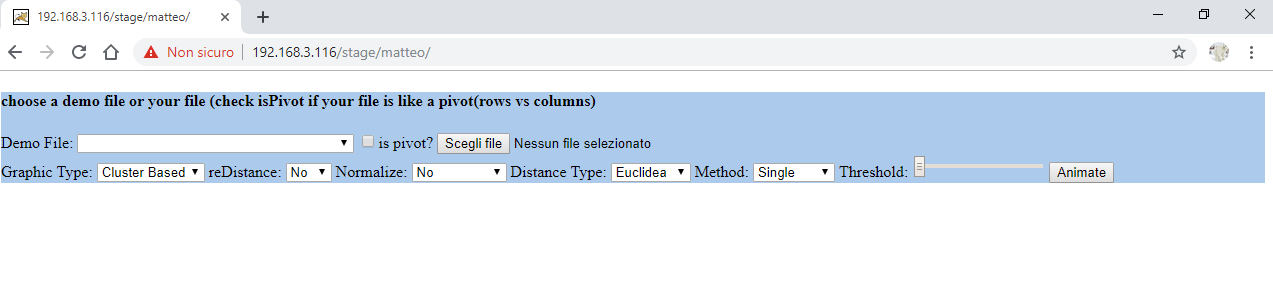
\includegraphics[width=1\linewidth]{./image/img-configurazione_reticolo.png}
	\caption{Configurazione usata nel sistema per generare il Reticolo della Conoscenza.}
	\label{Configurazione usata nel sistema per generare il Reticolo della Conoscenza.}
\end{figure}
\noindent

\subsection{Creazione dei file CSV}
\label{Creazione dei file CSV}
Come gi\`a accentato all'interno della sezione §\ref{Descrizione del sistema} prima di procedere alla creazione del Reticolo, ho dovuto preparare i dati di previsione. Questo \`e stato reso pi\`u agevole grazie alla creazione, da parte mia, di un metodo che ha il compito, una volta messa in funzione la Rete, di calcolare:
\begin{enumerate}
\item Le previsioni ottenibili da un vettore di previsione settato a 1 e -1 per ogni singolo elemento;
\item Sui dati del punto (1) un vettore delle differenze dove viene calcolato il delta in rapporto al vettore standard \footnote{Vettore tutto a zero}.
\end{enumerate}
\noindent
Il vettore delle differenze viene stampato su console del browser \footnote{unica alternativa facendo uso di solo codice javascript}, in modo che ne basti prelevare il contenuto e inserirlo su un file CSV. Ogni elemento per poter funzionare all'interno dell'applicativo deve essere separato da un ; e ogni riga di previsione deve essere preceduta dal codice della domande in modo da rendere pi\`u agevole l'interpretazione del Reticolo. \`E a discrezione dell'utente l'inserimento di un'ulteriore riga di dichiarazione dei parametri.

\subsection{Creazione del Reticolo della Conoscenza per sui dati di Prova}
\label{Creazione del Reticolo della Conoscenza per sui dati di Prova}

\subsubsection{L'architettura della Rete}
\label{L'architettura della Rete}
Durante la costruzione del Reticolo della Conoscenza \`e stato importante capire se effettivamente l'architettura scelta in precedenza fosse corretta, e il suo vero significato. La rete sviluppata per il progetto \`e una Rete neurale statica a multistrato, nella quale sono presenti i seguenti elementi:
\begin{itemize}
\item input layer: dove viene dichiarata la dimensione dell'input: lunghezza, larghezza e profondit\`a dei dati da analizzare;
\item hidden layer (o layer intermedio): composto da uno o p\`u strati nascosti (o intermedi) costituito da m neuroni;
\item output layer:  costituito da p neuroni pari al numero di output desiderati.
\end{itemize}
\noindent 
Una Rete neurale permette di formulare complessi modelli matematici (sistemi di equazioni differenziali ecc.) e di individuarne possibili soluzioni. Le soluzioni si determinano sempre a partire dai dati; tuttavia la scelta del modello\footnote{inteso come architettura.} \`e un'azione molto complessa.

L'architettura di Rete ipotizzata per i dati di prova e coerente con quanto affermato nella sezione \ref{Osservazioni su rete a 4 neuroni per 1 layer}, è il seguente:
\noindent
\begin{figure}[H]
\centering
	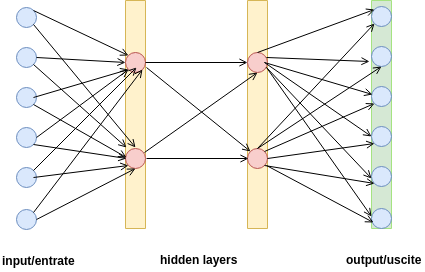
\includegraphics[width=0.60\linewidth]{./image/architettura-rete-prova.png}
	\caption{Architettura delle Rete di prova: 6 ingressi in una rete a 3 strati con 2 stati nascosti e 6 uscite.}
	\label{Archittettura delle Rete di prova: 6 ingressi in una rete a 3 strati con 2 stati nascosti e 6 uscite.}
\end{figure}
\noindent



\subsubsection{Reticolo della Conoscenza generato mediante previsioni sul set di dati che conto esclusivamente della conoscenza del candidato}
\label{Reticolo della Conoscenza generato mediante previsioni sul set di dati che tiene conto esclusivamente della conoscenza del candidato}

\noindent
\begin{figure}[H]
\centering
	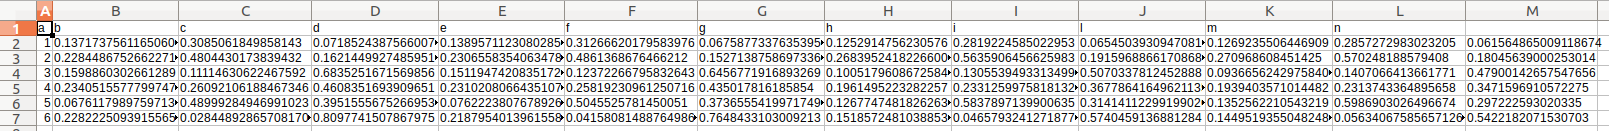
\includegraphics[width=1\linewidth]{./image/fileCSV_rete-prova.png}
	\caption{file CSV generato per la creazione del Reticolo della Conoscenza sui dati di prova.}
	\label{file CSV generato per la creazione del Reticolo della Conoscenza sui dati di prova.}
\end{figure}
\noindent
Di seguito sono riportate le sequenze di creazione del Reticolo della Conoscenza per i dati di prova che non risentono della probabilit\`a di indovinare di un candidato.
\noindent

\begin{figure}[H]
\centering
	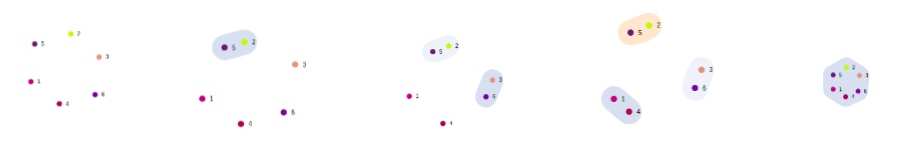
\includegraphics[width=1.20\linewidth]{./image/collage_reticolo-general-cluster.png}
	\caption{Reticolo della Conoscenza per i dati di prova - Cluster based.}
	\label{Reticolo della Conoscenza per i dati di prova - Cluster based.}
\end{figure}
\noindent

\begin{figure}[H]
\centering
	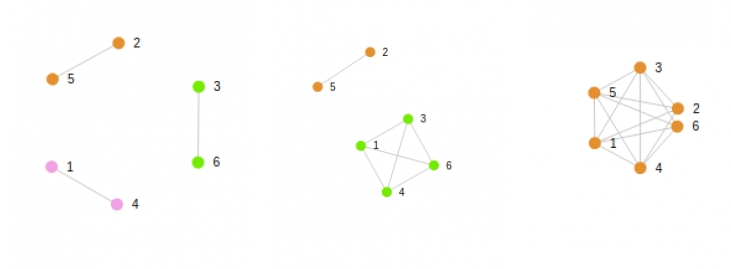
\includegraphics[width=1\linewidth]{./image/collage_reticolo-general-forced.png}
	\caption{Reticolo della Conoscenza per i dati di prova - Forced based.}
	\label{Reticolo della Conoscenza per i dati di prova - Forced based.}
\end{figure}
\noindent

\begin{figure}[H]
\centering
	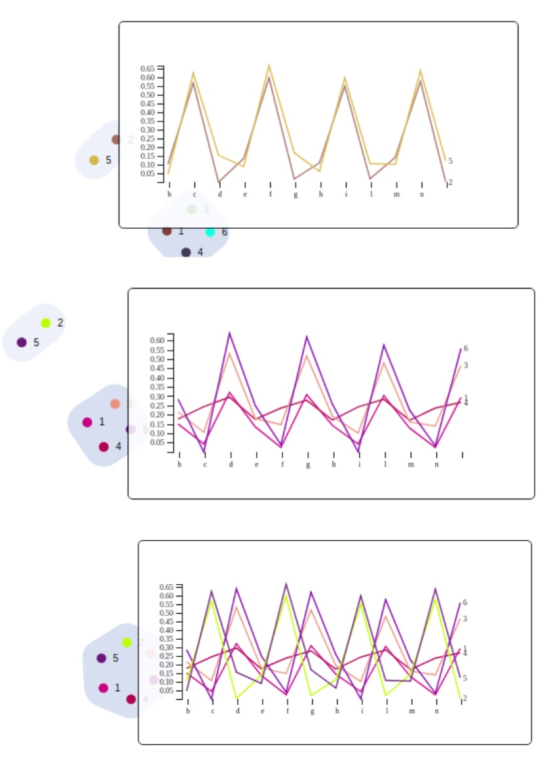
\includegraphics[width=0.50\linewidth]{./image/collage_reticolo-general-statistic.png}
	\caption{Reticolo della Conoscenza per i dati di prova - Statistiche.}
	\label{Reticolo della Conoscenza per i dati di prova - Statistiche.}
\end{figure}
\noindent
Appare come il Reticolo generato rispetta quando definito dalla figura \ref{Grafo rappresentante le relazioni esistenti tra il set di domande di prova.}.\\
Tuttavia effettuando delle ulteriori prove con file dati differenti; ma provenienti dalla medesima Rete neurale, ho riscontrato situazioni contrastanti. L'errore osservato nei casi non corretti riguarda le coppie di domande 1, 4 e 3, 6.\\\\
La spiegazione del Reticolo malformato \`e da ricondurre alla natura stessa dei vettori di input, usati per l'addestramento della Rete di prova. Difatti i valori delle domande correlate sono i medesimi, solo se entrambe le domande sono state poste in fase di test, altrimenti quando la domanda \`e non posta viene valutata 0. Questo provoca un'oscillazione degli accoppiamenti genitori-figli. Tuttavia \`e solo uno scostamento causato dall'occorrenza  con il quale le domande vengono poste, e di cui l'addestramento della Rete ne risente, come illustrato dalle figure seguenti.
\begin{figure}[H]
\centering
	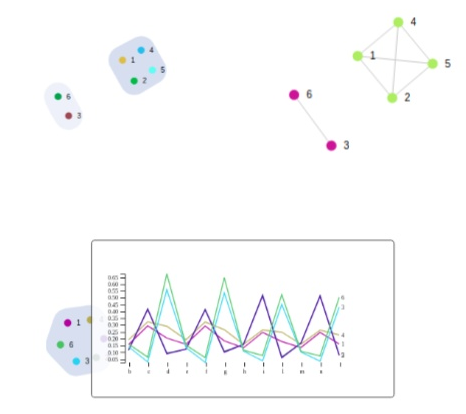
\includegraphics[width=0.60\linewidth]{./image/collage_reticolo-general-PROBLEMA.png}
	\caption{Reticolo della Conoscenza per i dati di prova - Presenza di valori di alterazione.}
	\label{Reticolo della Conoscenza per i dati di prova - Presenza di valori di alterazione.}
\end{figure}
\noindent
Le domande 6, 3 sono state poste un numero superiore di volte rispetto alle domande figlie 1, 4, per cui il sistema associa le coppie 1, 4 con le coppie 2, 5 che hanno tra loro una frequenza, dei valori iniziali, pi\`u vicina. Inoltre vi \`e da dire che il metodo Single usato dall'applicativo per associare le domande, nel momento in cui correla tra loro due punti, calcola il prossimo dal complessivo, invece che dal punto con una distanza appena superiore.\\
Per valutare al meglio l'impatto di quanto affermato sopra, in fase di test mi sono preoccupata di analizzare come si comporta la Rete neurale, relativa ai dati di prova, considerando esclusivamente la possibilit\`a che un candidato o risponda correttamente ad una domanda (1) o la sbagli (-1). I risultati di previsione ottenuti sono i seguenti:
\begin{figure}[H]
\centering
	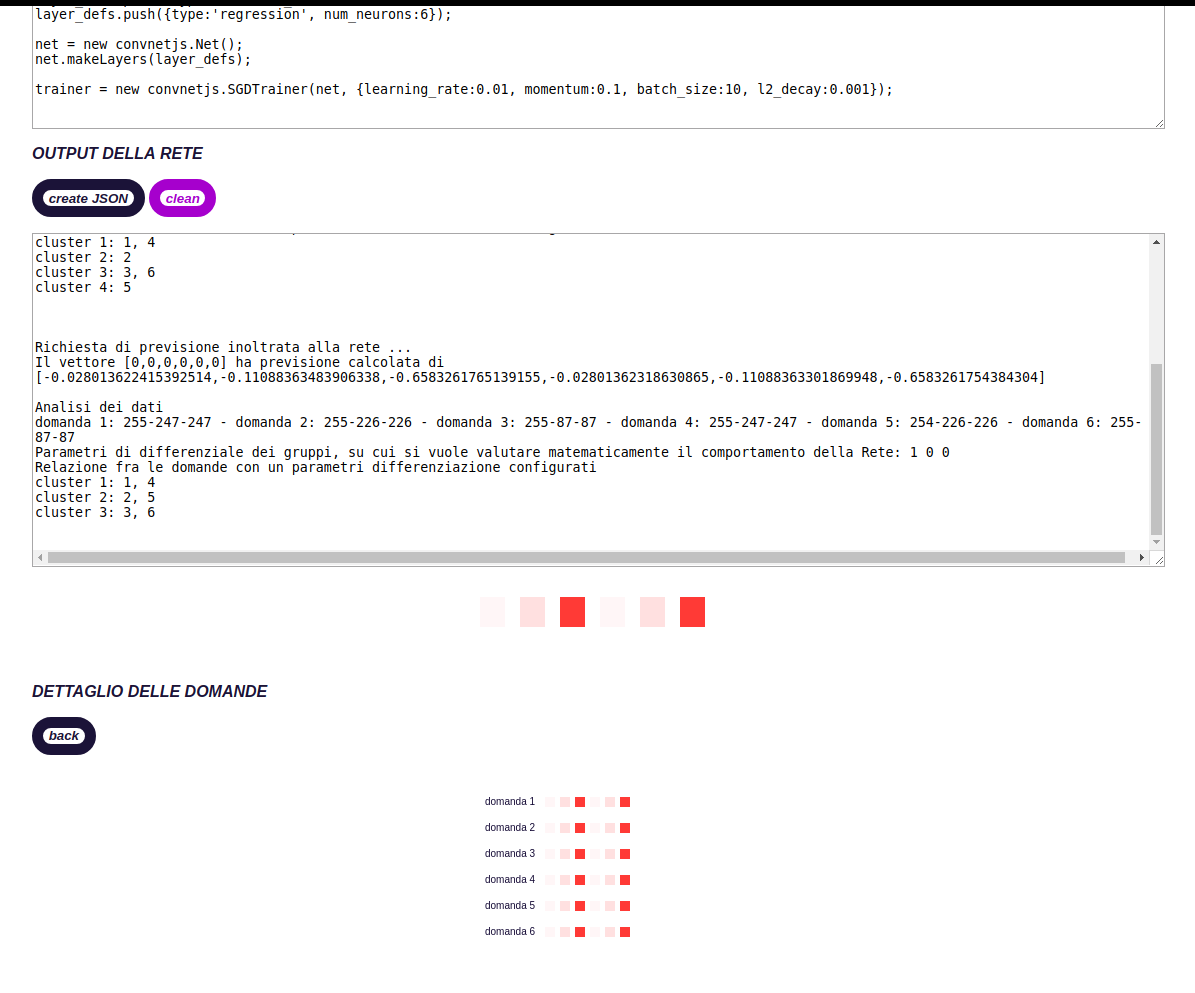
\includegraphics[width=1\linewidth]{./image/RetediProva_generatorinputpuro.png}
	\caption{Risultati della Rete di prova con un set di dati puro (esclusivamente 1 e -1).}
	\label{Risultati della Rete di prova con un set di dati puro (esclusivamente 1 e -1).}
	\end{figure}
	\noindent
Come si pu\`o vedere dalla figura \ref{Risultati della Rete di prova con un set di dati puro (esclusivamente 1 e -1).} le previsioni ottenute per le coppie di domande (1;4), (3;6) e (2;5) sono identiche, ad eccezioni di alcune variazioni impercettibili da ricondurre ad oscillazioni di Rete; e che non hanno alcun impatto sui risultati da raggiungere. Impostando di ottenere una previsione sul valore 0 e avendo allenato la Rete esclusivamente con valori -1 e 1 mi aspetto che venga effettuata la media, ed \`e quello che viene fatto effettivamente, per tutte le domande coinvolte.
Il fenomeno sorprendente, che mette in luce l'importanza di avere un valore 0 di risposta (non data) nel trainset, \`e mostrato nelle figure \ref{Risultati della Rete di test con un set di dati puro (esclusivamente 1 e -1), vettore previsione [-1, 0, 0, 0, 0, 0].} e  \ref{Risultati della Rete di test con un set di dati puro (esclusivamente 1 e -1), vettore previsione [0, 0, 0, -1, 0, 0].} sotto.
\begin{figure}[H]
\centering
	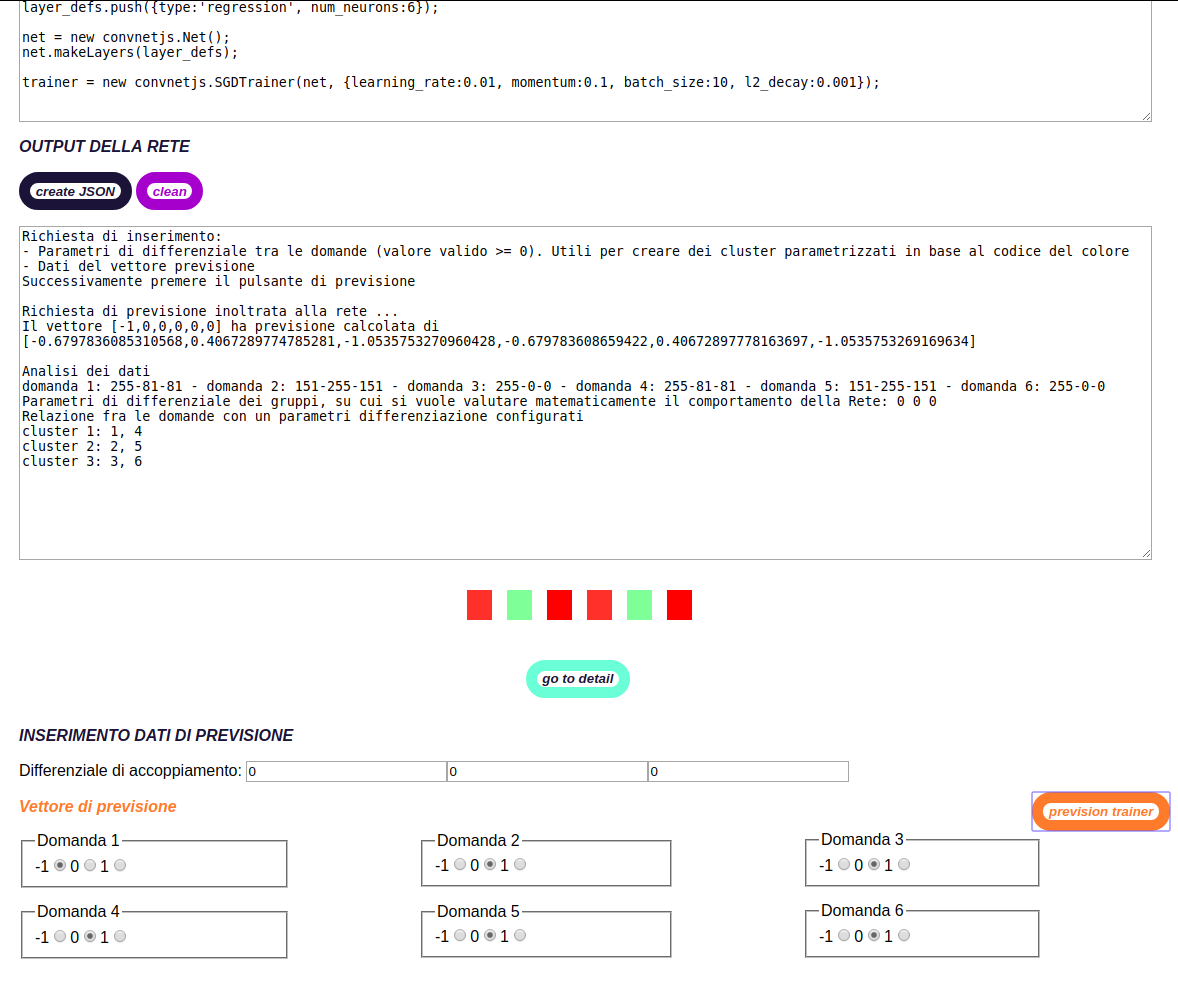
\includegraphics[width=1\linewidth]{./image/RetediProva_generatorinputpuro1.png}
	\caption{Risultati della Rete di test con un set di dati puro (esclusivamente 1 e -1), vettore previsione [-1, 0, 0, 0, 0, 0].}
	\label{Risultati della Rete di test con un set di dati puro (esclusivamente 1 e -1), vettore previsione [-1, 0, 0, 0, 0, 0].}
\end{figure}
\noindent

\begin{figure}[H]
\centering
	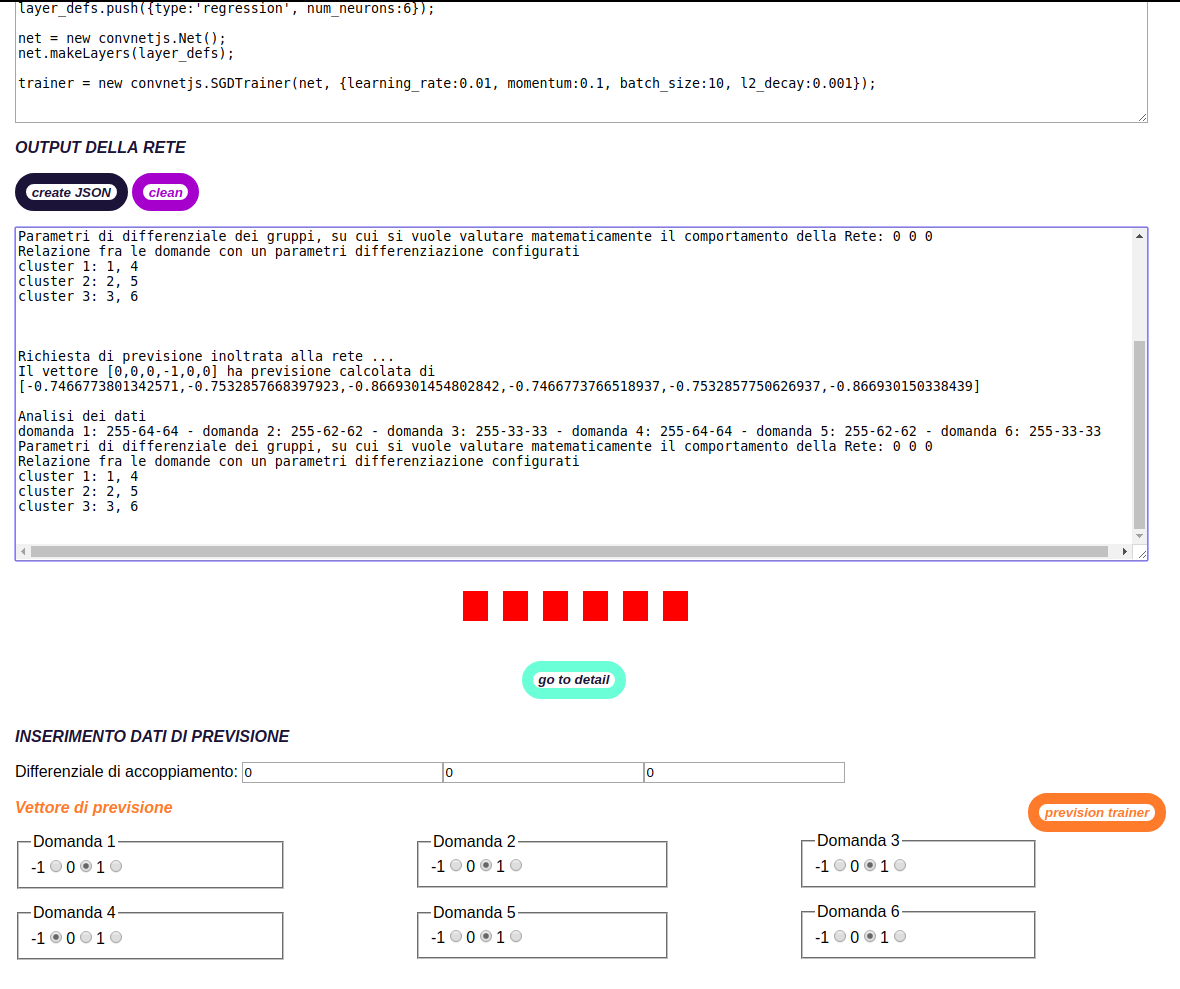
\includegraphics[width=1\linewidth]{./image/RetediProva_generatorinputpuro3.png}
	\caption{Risultati della Rete di test con un set di dati puro (esclusivamente 1 e -1), vettore previsione [0, 0, 0, -1, 0, 0].}
	\label{Risultati della Rete di test con un set di dati puro (esclusivamente 1 e -1), vettore previsione [0, 0, 0, -1, 0, 0].}
\end{figure}
\noindent
Non avere un valore a 0 porta le Rete a valutate come uniche relazioni, strette, esclusivamente quella tra la coppia coinvolta; rendendo meno possibile ogni altra assunzione sulle altre coppie \footnote{La presenza dello 0 mitiga questo aspetto.}. Ad esempio, le domande 2 e 4 vengono colorate di verdino nella previsione della domanda 1 e di rosso nella domanda 4. Questo ha un impatto negativo sia sulla previsione visiva della Rete, dal quale risulta impossibile la previsione di domande figlie e genitori, che nella costruzione del Reticolo della Conoscenza, in cui non può essere preso come valore di riferimento distanza 0.\\
La matrice correlazione ottenuta, tuttavia dal modello della PCA, risulta perfettamente allineata con le aspettative delle coppie di domande e delle previsioni, questo \`e possibile solo perch\`e i dati e le previsioni vengono valutati nella loro generalit\`a e non tra coppia di domande.


\subsubsection{Reticolo della Conoscenza generato mediante la frequenza calcolata sul set di dati che tiene conto esclusivamente della conoscenza del candidato}
\label{Reticolo della Conoscenza generato mediante la frequenza calcolata sul set di dati che tiene conto eclusivamente della conoscenza del candidato}
Ho ritenuto adeguato studiare il comportamento del set di dati anche in base alla frequenza; in modo da poterne valutare le differenze con la Rete neurale e quali siano, se esistenti, i benefici.\\
Come primo passo ho provveduto a calcolarmi, per ogni domanda, quale fosse la frequenza delle altre domande, valutate in accordo e in disaccordo con la risposta data. Ho effettuato il procedimento sia nel caso di una domanda con risposta correttamente che non.

\noindent
\begin{figure}[H]
\centering
	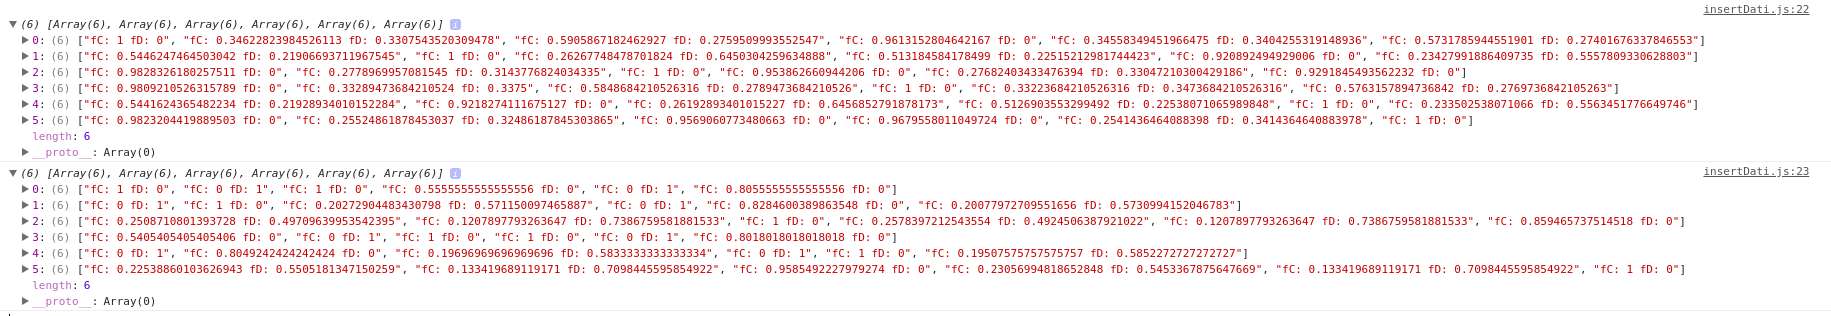
\includegraphics[width=1\linewidth]{./image/res_frequenceMatrix_OSS.png}
	\caption{Frequenza delle domande dei dati di test.}
	\label{Frequenza delle domande dei dati di test.}
\end{figure}
\noindent
L'immagine sopra illustra, per ogni domanda valutata a 1 (primo set di dati) e a -1 (secondo set di dati), la frequenza che intercorre in tutte le domande con segno coerente o opposto a quello della domanda in esame.
Il set di dati viene generato randomicamente con guida \footnote{con impiego del Grafo della Conoscenza (mostrato in figura \ref{Grafo rappresentante le relazioni esistenti tra il set di domande di prova.})}.
Analizzando i risultati di frequenza ottenuti, ho riscontrato i seguenti aspetti:
\begin{itemize}
\item Considerando i valori per riga:
\begin{itemize}
\item per le domande in cui le risposte si presentano a 1, i valori di frequenza che non rispettano le aspettative sono i seguenti:
\begin{itemize}
\item la domanda 3  con una frequenza correlata che coinvolge le coppie (1 ~ FC: 0.98, 3 ~ FC: 1) e (4 ~ FC: 0.95, 6 ~ FC: 0.98);
\item la domanda 6 con una frequenza correlata che coinvolge le coppie (1 ~ FC: 0.98, 6 ~ FC: 1) e (4 ~ FC: 0.96, 3 ~ FC: 0.95).
\end{itemize}
\item per le domande in cui le risposte si presentano a -1 i valori di frequenza che non rispetta le aspettative sono i seguenti:
\begin{itemize}
\item la domanda 1 con una frequenza correlata che coinvolge le coppie (1 ~ FC:1, 3 ~ FC:1) e (4 ~ FC:0.55, 6 ~ FC:0.80);
\item la domanda 4 con una frequenza correlata che coinvolge le coppie (4 ~ FC:1, 3 ~ FC:1) e (1 ~ FC:0.54, 6 ~ FC:0.80);
\end{itemize}
\end{itemize}
\item Considerando i valori per colonna:
\begin{itemize}
\item la domanda 1 si correla con la domanda 4;
\item la domanda 3 si correla con la domanda 6, 
\item la domanda 2 con la domanda 5.
\end{itemize}
\end{itemize}
\noindent
Tali considerazioni non sono esclusive per il singolo set di dati; ma rimangono costanti per ogni set di dati generato (anche se di natura parzialmente randomica). Ho riscontrato per ciascuna variabile al massimo un oscillazione che si attesta mai superiore a 0.2.
\\\\
I valori di frequenza possono concorrere alla formazione del Reticolo della Conoscenza. Per renderlo possibile ho provveduto ha creare un file csv, che contenesse per ognuna delle domande, tutte le domande coinvolte valutate con frequenze positive e negative correlate e opposte. La tecnica permette la generazione, per ogni domanda, di un vettore contenente un quantit\`a di dati 4 volte la dimensione dell'input/output della Rete.
Il divario permette, positivamente, di poter costruire un Reticolo ove i dati per ogni nodo hanno una stabilit\`a concreta.\\
Tuttavia il Reticolo generato riscontra delle peculiarit\`a:
\begin{itemize}
\item la frequenza non effettua alcuna riduzione dimensionale provocando un utilizzo di spazio pari al numero di domande/dati da analizzare. Ci\`o comporta che per grandi moli di dati lo spazio necessario cresce in maniera elevata rispetto al numero di elementi di input;
\item la frequenza funziona male sui valori anomali.
\end{itemize}
\noindent
Il divario tra i valori per riga e colonna sono legittimati dalla natura del set di valori di input. In esso sono contenuti valori 0, e non esclusivamente -1 e 1, causa diretta dell'oscillazione delle correlazioni strette esistenti tra le domande accoppiate \footnote{per i dati di prova le domande accoppiate sono (1;4), (3;6) e (2;5)}.\\\\
\noindent
Il Reticolo generato rispetta fedelmente le aspettative, definite dal Grafo della Conoscenza in figura \ref{Grafo rappresentante le relazioni esistenti tra il set di domande di prova.}. Tuttavia questo non va valutato come un risultato positivo, in quanto indicatore che ai valori 0, che dovrebbero alterare, anche se marginalmente il risultato finale viene data la medesima importanza non tenendo conto del numero di occorrenze (dimostrazione di come la frequenza gestisce male i valori anomali - vedi esempio sotto). Il beneficio dell'uso della Rete sta proprio in quest'ultimo fattore, con l'impiego dell'apprendimento vengono rilevate situazioni che la sola frequenza non \`e in grado di pesare.


\begin{verbatim}
------------------------------------------------------
Esempio che mette in rapporto la frequenza con le 
previsioni di una Rete neurale

Analisi della risposta positiva (FC):
(1) 1/1 = 1,  1 risposta positiva tra tutte le domande (=1),
 che sono accoppiate con la domanda i, quando viene risposta
correttamente	
(2) 8/8 = 1, 8 risposte positive tra tutte le domande (=8),
che sono accoppiate con la domanda i + 1, quando viene risposta
correttamente

- Per la frequenza: n e n + 1 hanno il medesimo valore di FC
- Per una Rete neurale: un evento che si verifica 1 volta e
un evento che si verifica 8 volte hanno un peso differente,
questo perché una rete effettua previsioni non su dati
statistici, ma per mezzo di train.
-------------------------------------------------------
\end{verbatim}


\begin{figure}[H]
\centering
	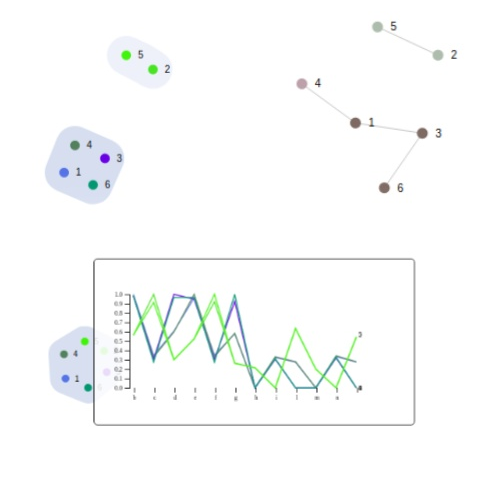
\includegraphics[width=0.50\linewidth]{./image/collage_reticolo-general-FREQ.png}
	\caption{Reticolo della Conoscenza per i dati di prova - Frequenza.}
	\label{Reticolo della Conoscenza per i dati di prova - Frequenza.}
\end{figure}
\noindent


\subsubsection{Osservazioni sul Reticolo generato dalle previsioni della rete}
\label{Osservazioni generato dalla previsioni della rete}
In conclusione il Reticolo della Conoscenza, costruito per mezzo delle previsioni della Rete neurale, anche se non sempre perfettamente coerente con le aspettative; nella maggioranza dei casi ricalca fedelmente quanto evidenziato nella figura \ref{Grafo rappresentante le relazioni esistenti tra il set di domande di prova.} nella sezione § \ref{Test effettuati}. \\
Quando il Reticolo non \`e soggetto a deviazioni, gli accoppiamenti tra i punti, rispettano quanto dichiarato dalla matrice correlazione ottenuta dal modello generato dall'uso della PCA, e visibile dall'immagine \ref{CSV generato a partire dalla matrice correlazione del set della rete di prova.}.
\`E obbligo precisare, tuttavia che i risultati della PCA non devono essere presi come assioma assoluto. Le argomentazioni sono le seguenti:
\begin{itemize} 
\item La Rete neurale, pu\`o cogliere oscillazioni che il modello matematico non \`e in grado, e questo va ad invalidare i risultati ottenuti non solo dalla matrice correlazione, ma anche dell'individuazione dei punti sulle prime due componenti;
\item La PCA, come si \`e visto accadere con la frequenza, non tiene conto del numero di volte cui si verifica un evento, attribuendone il medesimo peso. Invece la Rete, neurale mediante apprendimento, riesce a valutare al meglio, tali fenomeni, avvicinandosi il pi\`u possibile alla realt\`a.
\item Lo scopo principale della PCA \`e quello di spostare gli assi di rappresentazione degli eventi; in modo che vi sia una maggiore facilit\`a di comprensione dei dati, come si ha con la standardizzazione dei valori.
\end{itemize}

\subsubsection{Reticolo della Conoscenza generato con set di dati che tiene conto della possibilit\`a che un candidato ha di indovinare la risposta}
\label{Reticolo della Conoscenza generato con set di dati che tiene conto della possibilita che un candidato ha di indovinare la risposta}
Sia che si tratti di una valutazione per frequenza, che di previsioni ottenute dalla Rete neurale, il Reticolo tende ad ogni nuovo set di dati, ad assumere una diversa conformazione, che ne rende difficile trarne delle conclusioni.
In linea generale, si pu\`o affermare che:
\begin{itemize}
\item Le domande figlie e le domande genitori vengono sempre raggruppate in un singolo insieme, prima di venire fuse in un unico cluster, assieme alle domande con cui non esiste correlazione;
\item Il Reticolo della Conoscenza generato con le previsioni della Rete, rispetta meglio le oscillazioni introdotte dalla possibilit\`a di indovinare. Difatti, come vale per il valore 0, la frequenza si dimostra poco capace di cogliere le discrepanze dal modello, non riuscendo a dare il giusto peso ai valori anomali.
\end{itemize}

\begin{figure}[H]
\centering
	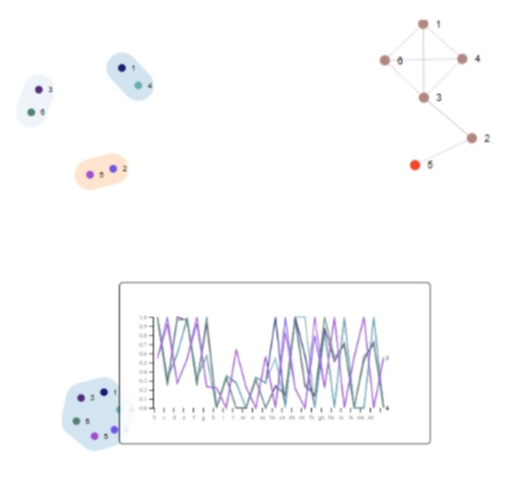
\includegraphics[width=0.60\linewidth]{./image/collage_reticolo-probability-FREQ.png}
	\caption{Reticolo della Conoscenza per i dati di prova con indovinato - Frequenza.}
	\label{Reticolo della Conoscenza per i dati di prova con indovinato - Frequenza.}
\end{figure}
\noindent
\begin{figure}[H]
\centering
	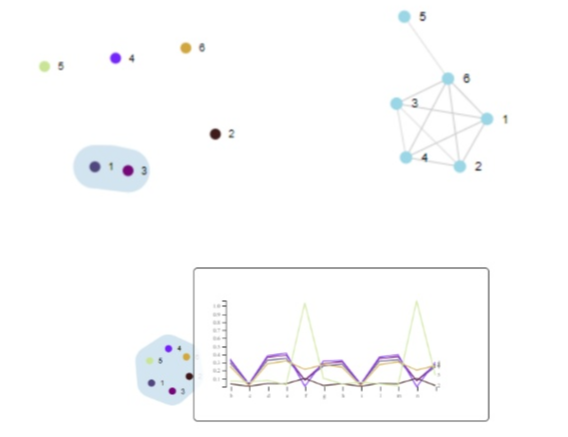
\includegraphics[width=0.60\linewidth]{./image/collage_reticolo-probability.png}
	\caption{Reticolo della Conoscenza per i dati di prova con indovinato - Previsioni.}
	\label{Reticolo della Conoscenza per i dati di prova con indovinato - Previsioni.}
\end{figure}
\noindent


\subsection{Creazione del Reticolo della Conoscenza per le domande di logica nel database}
\label{Creazione del Reticolo della Conoscenza per le domande di logica nel database}

Requisiti da assolvere, per costruire un Reticolo della Conoscenza valido per le domande contenute nel database aziendale:
\begin{enumerate}
\item Studio del testo delle domande per individuare quali sono i gruppi di argomenti;
\item Formulazione di una buona architettura, avvalendosi della grandezza del set di dati, del numero di domande e della conoscenza di quanto emerso dal punto (1);
\item Validazione dei risultati ottenuti, confrontando i cluster con gli argomenti identificati al punto (1). Si deve tenere conto che non si potrà mai ottenere un match perfetto, in quanto il set risente della probabilità di indovinare.
\end{enumerate}


\subsubsection{Individuazione dei gruppi di argomenti}\mbox{}
\label{Individuazione dei gruppi di argomenti 89}
Le domande di logica si compongono di due macro-argomenti principali:
\begin{itemize}
\item Domande sulle Serie numeriche;
\item Domande su diagrammi di Eulero-Venn.
\end{itemize}
\noindent
Le restanti domande non presentano un argomento specifico, risultando complesse da catalogare. Queste ultime le ho valutate come punti isolati.
\\
\noindent
Di seguito, in forma tabellare viene riportata la categorizzazione delle domande.
\begin{longtable}{|c|c|}
	\hline
	\textbf{Codice} & \textbf{Argomento} \\\hline\hline

aelkshwnzj & Nessuno \\
bajsownqty & Nessuno \\
bdwjgxtdsm & Nessuno \\
bfmfxcudzq & Nessuno \\
bkfstjjeaw & Nessuno \\
bojihohutw & Nessuno \\
ccsofpywab & Eulero-Venn \\
cfkjhtcjjp & Nessuno \\
cfxigdfgsu & Eulero-Venn \\
cidpdlimnu & Nessuno \\
cxjganjqsl & Nessuno \\
cxwrjrltfv & Nessuno \\
diucioyoxo & Nessuno \\
dpzaqasqro & Nessuno \\
ectvbesohs & Nessuno \\
efbcntiwcr & Nessuno \\
elbottcdse & Nessuno \\
fbekkymdja & Nessuno \\
fclxhnodej & Nessuno \\
flsdkdhwpz & Nessuno \\
fpiajgnnfb & Nessuno \\
fupxesqveq & Nessuno \\
fvwcpjdfai & Nessuno \\
gilviisrcb & Eulero-Venn \\
gxushjkzth & Nessuno \\
hacwlyvymr & Nessuno \\
heohdfuqpi & Nessuno \\
heusbnnnto & Nessuno \\
hxsywnmxdd & Nessuno \\
iesmuuktcs & Nessuno \\
ifrcopoblv & Nessuno \\
iojsfvnpii & Nessuno \\
islhstwuay & Nessuno \\
jgcxaxgrrw & Nessuno \\
jnxymdjdxl & Nessuno \\
jomkrqdwwr & Nessuno \\
jwvreihjvv & Nessuno \\
jygnlagbhv & Nessuno \\
kkhcmynavp & Nessuno \\
kprsxjkubz & Serie numeriche \\
kzorhoohrb & Nessuno \\
lhuxxlqtyz & Nessuno \\
ljypeljfkh & Eulero-Venn \\
lqyvhqfmqd & Nessuno \\
lrqrblychp & Nessuno \\
mfycpmjyzc & Nessuno \\
mhaimflmrt & Eulero-Venn \\
mnrnuysydx & Serie numeriche \\
ngtquzulpk & Nessuno \\
nrawevuhkv & Nessuno \\
oaszeadbqh & Nessuno \\
obwqtgpxek & Eulero-Venn \\
okklvldqlc & Nessuno \\
osvluiqhbp & Nessuno \\
pfctjunpxs & Serie numeriche \\
pfsvqgsfen & Serie numeriche \\
poiuytrewq & Eulero-Venn \\
ptfkuubpyy & Nessuno \\
ptwccskjcf & Serie numeriche \\
pxvpfrjqnb & Serie numeriche \\
qbnjsxmnxx & Serie numeriche \\
qfxndoiusk & Nessuno \\
qmzlhizqng & Nessuno \\
qsqbqjczyv & Eulero-Venn \\
ribhqompcp & Nessuno \\
sucpsfikqd & Nessuno \\
tnmucbefiy & Nessuno \\
tocsjuegmj & Nessuno \\
tpfgrbtdur & Nessuno \\
ukafbvkjxl & Nessuno \\
ungslccrdw & Serie numeriche \\
uoohruqjig & Serie numeriche \\
uoztprdkre & Nessuno \\
upmqfdzqqd & Nessuno \\
voqwkjnxuv & Eulero-Venn \\
vtjiowgfxp & Nessuno \\
wfthuqobvv & Nessuno \\
wpfhnhktzw & Nessuno \\
wqkhvmdpol & Serie numeriche \\
xmqopkamew & Serie numeriche \\
xnyfhvvlzx & Serie numeriche \\
xvbullwvol & Nessuno \\
yxkoznnxis & Nessuno \\
zcflqcwpgh & Nessuno \\
zegfndrnwr & Nessuno \\
zptjzdwilf & Nessuno \\
zqrfurehmz & Serie numeriche \\
zrehhcvjyl & Serie numeriche \\
zvlwoledbc & Eulero-Venn \\
\hline
	
\caption{Gruppi di argomento per le domande di logica}\label{tab:Gruppi di argomento per le domande di logica}
\end{longtable}

\subsubsection{Architettura della Rete testata}
\label{Architettura della Rete testata 89}
Come già visto all'interno di §\ref{Rete neurale}, la scelta dell'architettura adatta per una rete che deve trattare una grande mole di dati e di cui non si ha piene conoscenza del risultato finale perché soggetti all'indovinato come visto in §\ref{PCA} rende tale compito molto arduo.\\
L'unico modo che ho individuato per affrontare il problema, è procedere con l'analisi del set di dati in input aiutandomi con le conoscenze acquisite durante la costruzione del Reticolo sul set di prova.\\\\
\noindent
Ho testato gli effetti sulla Rete e sulla generazione del Reticolo, di una molteplicit\`a di architetture. Le pi\`u rilevanti sono le seguenti:
\begin{itemize}
\item \begin{verbatim}
layer_defs = [];
layer_defs.push({type:'input', out_sx:1, out_sy:1, out_depth:89});
layer_defs.push({type:'fc', num_neurons:12, activation: 'tanh'});
layer_defs.push({type:'fc', num_neurons:12, activation: 'tanh'});
layer_defs.push({type:'regression', num_neurons:89});
        
net = new convnetjs.Net();
net.makeLayers(layer_defs);
trainer = new convnetjs.SGDTrainer(net, {learning_rate:0.01, 
momentum:0.1, batch_size:10, l2_decay:0.001});
\end{verbatim}
\noindent
Per formulare la configurazione sopra espressa, ho preso come riferimento l'architettura della Rete di prova e ne ho modificato il numero di neuroni per layers, sulla base del aumento del numero di domande e sulla diminuzione del numero di entry nel set di dati di logica. Non posso essere attesi risultati eccelsi, in quanto non vengono considerati il numero di cluser possibili, ma è una buona base di partenza per le osservazioni.
\item \begin{verbatim}
layer_defs = [];
layer_defs.push({type:'input', out_sx:1, out_sy:1, out_depth:89});
layer_defs.push({type:'fc', num_neurons: 4, activation: 'tanh'});
layer_defs.push({type:'fc', num_neurons: 4, activation: 'tanh'});
layer_defs.push({type:'fc', num_neurons:10, activation: 'tanh'});
layer_defs.push({type:'regression', num_neurons:89});
        
net = new convnetjs.Net();
net.makeLayers(layer_defs);
trainer = new convnetjs.SGDTrainer(net, {learning_rate:0.01, 
momentum:0.1, batch_size:10, l2_decay:0.001});
\end{verbatim}

\item \begin{verbatim}
layer_defs = [];
layer_defs.push({type:'input', out_sx:1, out_sy:1, out_depth:89});
layer_defs.push({type:'fc', num_neurons: 2, activation: 'tanh'});
layer_defs.push({type:'fc', num_neurons: 4, activation: 'tanh'});
layer_defs.push({type:'fc', num_neurons:10, activation: 'tanh'});
layer_defs.push({type:'regression', num_neurons:89});
        
net = new convnetjs.Net();
net.makeLayers(layer_defs);
trainer = new convnetjs.SGDTrainer(net, {learning_rate:0.01, 
momentum:0.1, batch_size:10, l2_decay:0.001});
\end{verbatim}

\item \begin{verbatim}
layer_defs = [];
layer_defs.push({type:'input', out_sx:1, out_sy:1, out_depth:89});
layer_defs.push({type:'fc', num_neurons: 4, activation: 'tanh'});
layer_defs.push({type:'fc', num_neurons: 4, activation: 'tanh'});
layer_defs.push({type:'fc', num_neurons: 5, activation: 'tanh'});
layer_defs.push({type:'fc', num_neurons: 5, activation: 'tanh'});
layer_defs.push({type:'regression', num_neurons:89});
        
net = new convnetjs.Net();
net.makeLayers(layer_defs);
trainer = new convnetjs.SGDTrainer(net, {learning_rate:0.01, 
momentum:0.1, batch_size:10, l2_decay:0.001});
\end{verbatim}
\end{itemize}

\paragraph{Prima architettura: layers(12, 12)}\mbox{}\\\\
\label{Prima architettura}
\noindent
Il Reticolo della Conoscenza generato è il seguente:
\begin{figure}[H]
\centering
	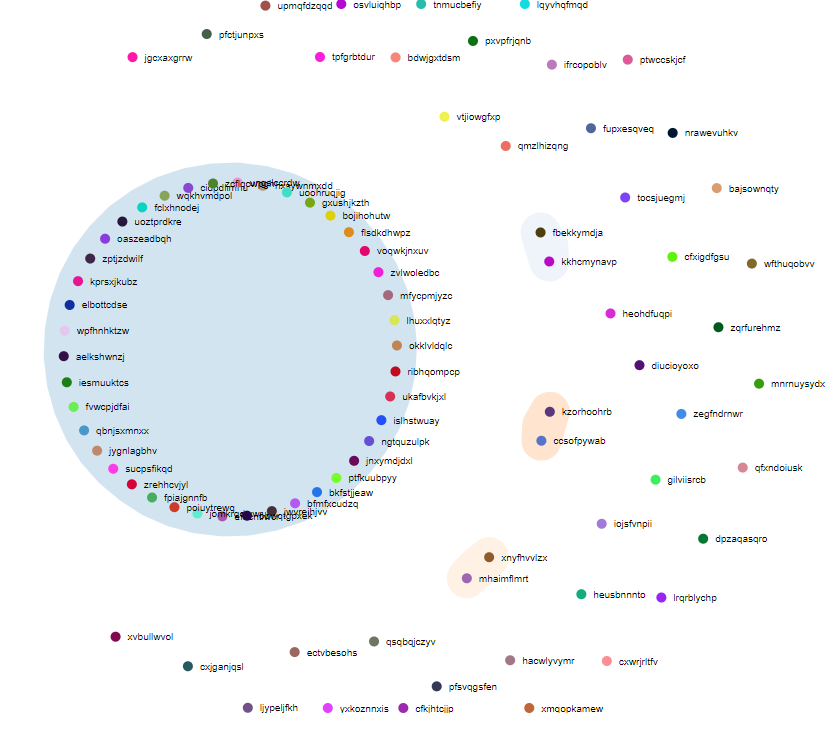
\includegraphics[width=0.70\linewidth]{./image/logica(12,12).png}
	\caption{Reticolo della Conoscenza layers(12, 12) - Cluster Based.}
	\label{Reticolo della Conoscenza layers(12, 12) - Cluster Based.}
\end{figure}
\noindent

\begin{figure}[H]
\centering
	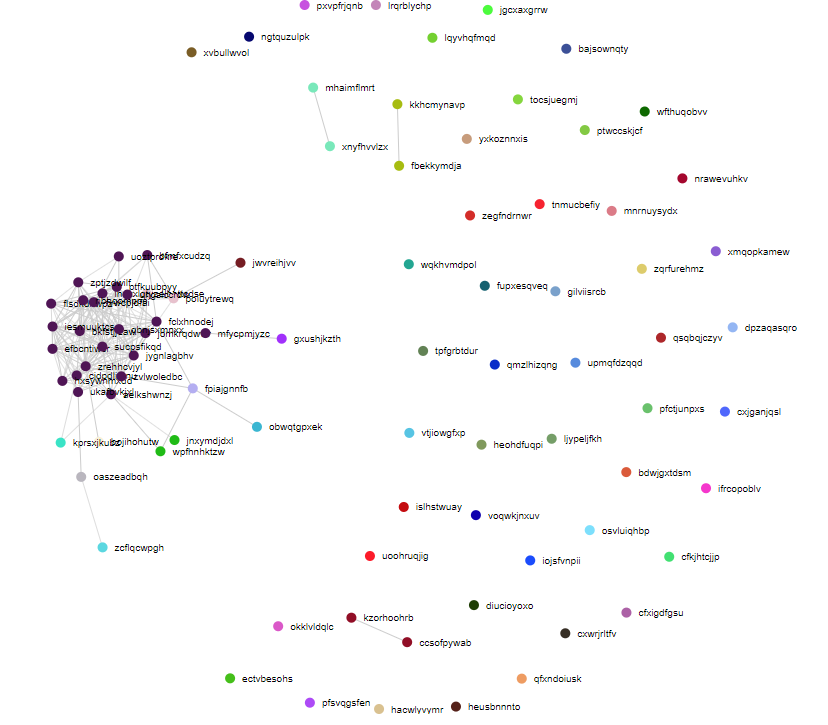
\includegraphics[width=0.70\linewidth]{./image/logica(12,12)_forced.png}
	\caption{Reticolo della Conoscenza layers(12, 12) - Forced Based.}
	\label{Reticolo della Conoscenza layers(12, 12) - Forced Based.}
\end{figure}
\noindent

\begin{figure}[H]
\centering
	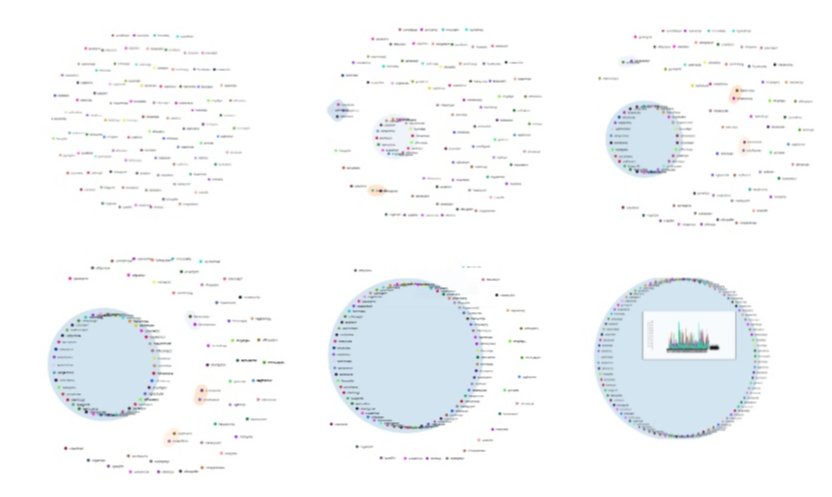
\includegraphics[width=0.70\linewidth]{./image/collage_reticolo-logica(12,12).png}
	\caption{Sequenza di creazione del Reticolo della Conoscenza layers(12, 12) - Cluster Based.}
	\label{Sequenza di creazione del Reticolo della Conoscenza layers(12, 12) - Cluster Based.}
\end{figure}
\noindent
\subparagraph{Osservazioni dei risultati}\mbox{}
\noindent
Prima di tutto si crea un unico cluster, e non due come era atteso, però si vanno ad insinuare un buon numero delle domande sulle Serie numeriche e su Eulero Venn. Tuttavia le domande dello stesso argomento non sono le prime a correlarsi.
\begin{longtable}{|c|c|}
	\hline
	\textbf{Serie numeriche} & \textbf{Eulero Venn} \\\hline\hline
	kprsxjkubz & obwqtgpxek \\
	qbhjsxmnxx & poiuytrewq \\
	ungslccrdw & voqwkjnxuv \\ 
	uoohruqjig & zvlwoledbc \\
	wqkhvmdpol & \\
	zrehhcvjvl & \\
\hline
\caption{Domande contenute nel primo cluster}\label{tab:Domande contenute nel primo cluster}
\end{longtable}
\noindent
Le domande correlate nei cluster \textit{(mhaimflmrt, xnyfhvvlzx)}, \textit{(ccsofpywab, kzorhoohrb)} e \textit{(fbekkymdja, kkhcmynavp)}, visibili in tabella \ref{Reticolo della Conoscenza layers(12, 12) - Cluster Based.}  non presentano alcuna analogia tematica. \\
Riducendo la correlazione tra i cluster si generano 2 cluster, come visibili dalla tabella \ref{Sequenza di creazione del Reticolo della Conoscenza layers(12, 12) - Cluster Based.}; ma nuovamente non viene rispettata la differenziazione tra domande Serie numeriche e Eulero Venn.\\\\
A seguito di numerosi test che sono succeduti a questa prima configurazione, ho potuto confermare quanto avevo gi\`a intuito in precedenza, e descritto in §\ref{Architetture testate}: un numero superiore di 11 neuroni genera una situazione di overfitting delle previsioni della Rete.

\paragraph{Seconda architettura: layers(4, 4, 10)}\mbox{}\\\\
\label{Seconda architettura}
\noindent
Il Reticolo della Conoscenza generato è il seguente:
\begin{figure}[H]
\centering
	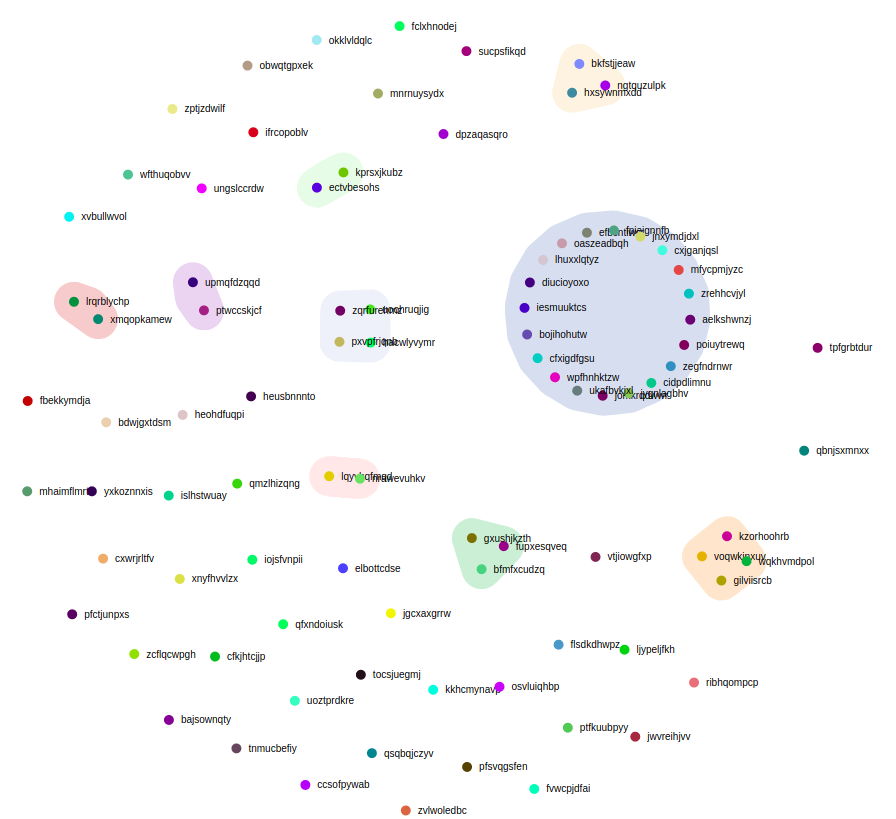
\includegraphics[width=0.70\linewidth]{./image/logica(4,4,10).png}
	\caption{Reticolo della Conoscenza layers(4, 4, 10) - Cluster Based.}
	\label{Reticolo della Conoscenza layers(4, 4, 10) - Cluster Based.}
\end{figure}
\noindent

\begin{figure}[H]
\centering
	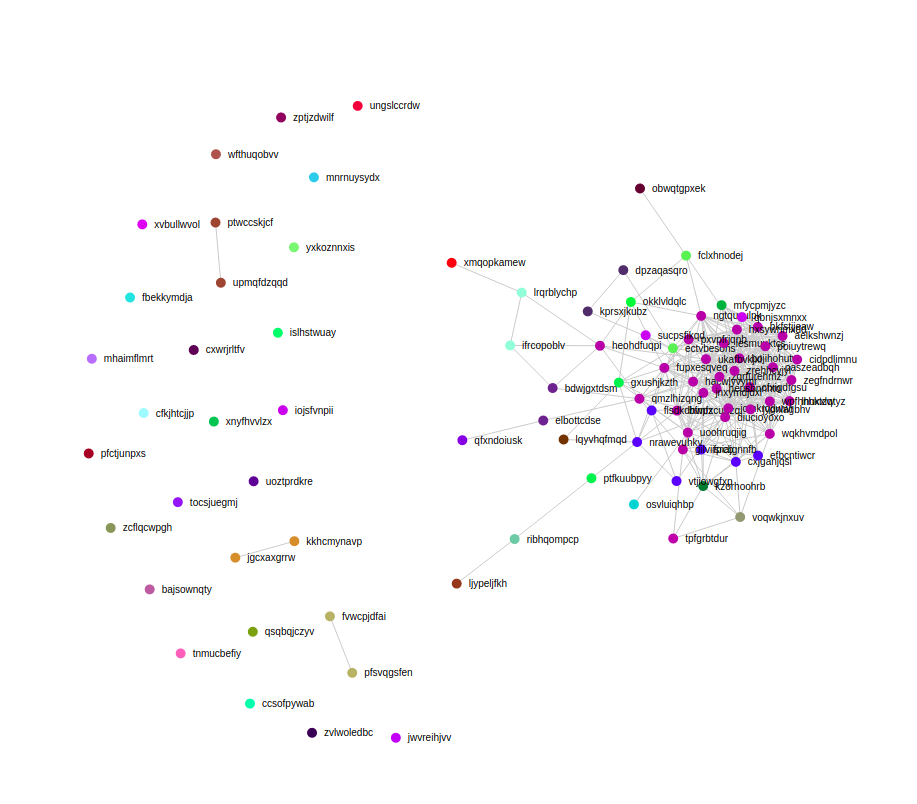
\includegraphics[width=0.70\linewidth]{./image/logica(4,4,10)_forced.png}
	\caption{Reticolo della Conoscenza layers(4, 4, 10) - Forced Based.}
	\label{Reticolo della Conoscenza layers(4, 4, 10) - Forced Based.}
\end{figure}
\noindent

\begin{figure}[H]
\centering
	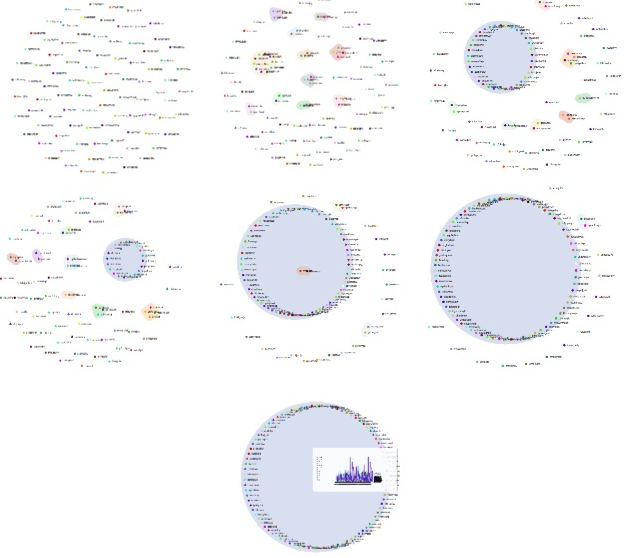
\includegraphics[width=0.70\linewidth]{./image/collage_reticolo-logica(4,4,10).png}
	\caption{Sequenza di creazione del Reticolo della Conoscenza layers(4, 4, 10) - Cluster Based.}
	\label{Sequenza di creazione del Reticolo della Conoscenza layers(4, 4, 10) - Cluster Based.}
\end{figure}
\noindent
\subparagraph{Osservazioni dei risultati}\mbox{}
\label{Osservazioni dei risultati}
Questo, ha mio avviso \`e, uno dei Reticolo pi\`u interessanti che ho generato, sulle domande di logica.
Esiste un cluster principale e una decina di gruppi di dimensione via via sempre minore. A mano a mano che viene incrementata la threshold, i gruppi vengono inglobati dal gruppo principale. I punti isolati sono in numero notevole, come si pu\`o vedere dalla figura \ref{Reticolo della Conoscenza layers(4, 4, 10) - Cluster Based.} anche se la thresehold di competenza \`e gi\`a quasi a met\`a del suo percorso.\\
Questi punti isolati rappresentano, nella maggioranza dei casi, tutte quelle domande che non trovano correlazione n\`e tra le serie numeriche, n\`e tra i diagrammi di Eulero-Venn.\\
Nel cluster principale vengono posizionati i seguenti punti:
\begin{longtable}{|c|c|}
	\hline
	\textbf{Serie Numeriche} & \textbf{Eulero-Venn} \\\hline\hline
	zrehhcvjyl & cfxigdfgsu \\
	           & poiuytrewq \\
	
\hline
\caption{Domande contenute nel primo cluster (blu)}\label{tab:Domande contenute nel primo cluster}
\end{longtable}
\noindent
Ci sono tuttavia anche altri cluster interessanti:
\begin{longtable}{|c|c|}
	\hline
	\textbf{Serie Numeriche} & \textbf{Eulero-Venn} \\\hline\hline
	wqkhmdpol & gilviisrcb \\
	           & voqwkijnxuv\\
	
\hline
\caption{Domande contenute nel secondo cluster (rosetta)}\label{tab:Domande contenute nel secondo cluster}
\end{longtable}
\noindent

\begin{longtable}{|c|c|}
	\hline
	\textbf{Serie Numeriche} & \textbf{Eulero-Venn} \\\hline\hline
	zqrtfurehmz &  \\
	uoohruqjiq  & \\
	zqrtfurehmz & \\
	
\hline
\caption{Domande contenute nel terzo cluster (blu chiaro)}\label{tab:Domande contenute nel terzo cluster}
\end{longtable}
\noindent
Il primo e il secondo cluster hanno una predominanza delle domande, per quanto concerne le domande catalogate, su Eulero-Venn; e il terzo per le domande sulle Serie numeriche.\\
I tre gruppi molto probabilmente hanno difficolt\`a superiori per un candidato e per questo vengono inglobati uno dentro l'altro passo passo.
Prima di tutto il primo cluster, influenzato dai dati di probabilit\`a, ingloba il terzo cluster e successivamente il secondo (la domanda \textit{zqrtfurehmz} per un candidato non allenato pu\`o risultare pi\`u complessa rispetto alla domanda \textit{zrehhcvjyl}).

\paragraph{Terza architettura: layers(2, 4, 10)}\mbox{}\\\\
\label{Terza architettura}
\noindent
I risultati sono di poco discostanti, rispetto ai risultati ottenuti dalla configurazione a layers (4, 4, 10). Di seguito riporto esclusivamente la generazione del Reticolo.

\begin{figure}[H]
\centering
	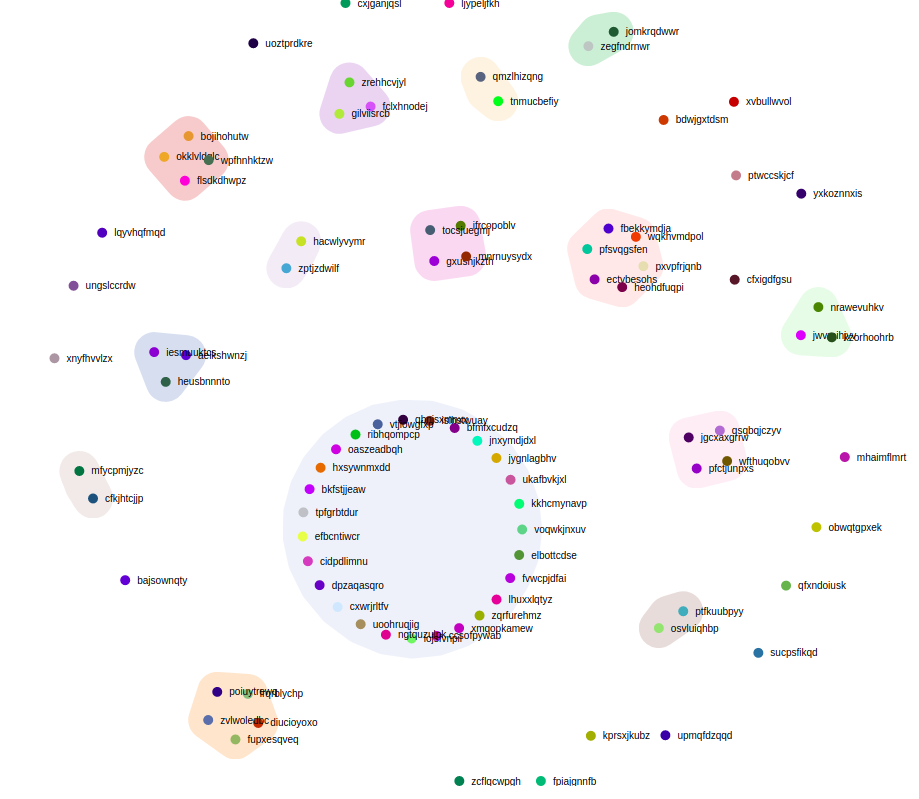
\includegraphics[width=0.70\linewidth]{./image/logica(2,4,10).png}
	\caption{Reticolo della Conoscenza layers(2, 4, 10) - Cluster Based.}
	\label{Reticolo della Conoscenza layers(2, 4, 10) - Cluster Based.}
\end{figure}
\noindent

\begin{figure}[H]
\centering
	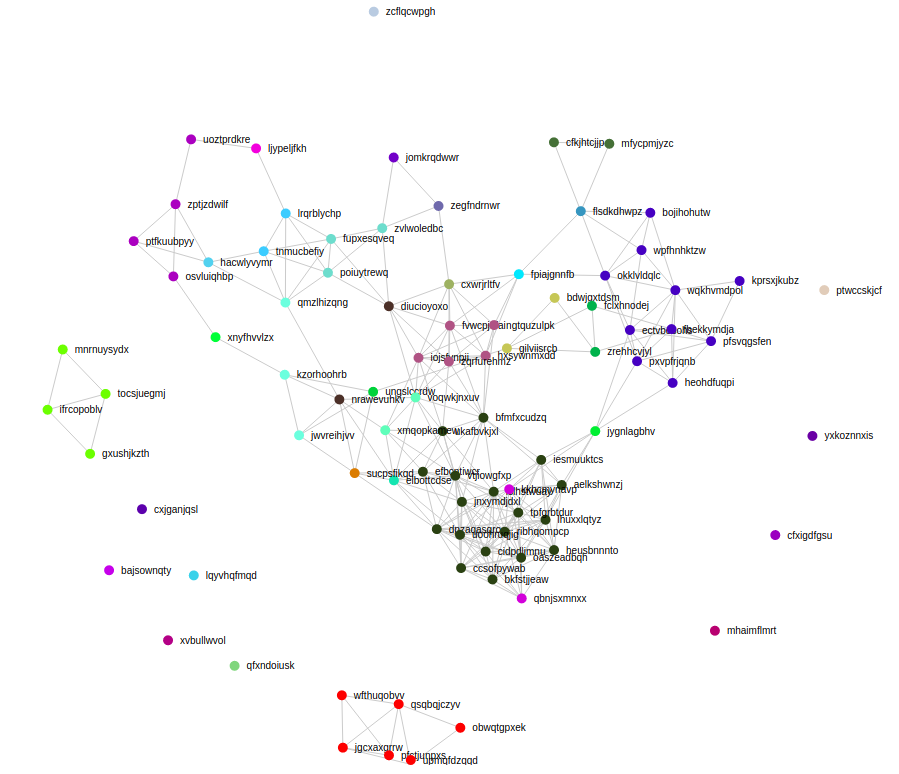
\includegraphics[width=0.70\linewidth]{./image/logica(2,4,10)_forced.png}
	\caption{Reticolo della Conoscenza layers(2, 4, 10) - Forced Based.}
	\label{Reticolo della Conoscenza layers(2, 4, 10)) - Forced Based.}
\end{figure}
\noindent

\begin{figure}[H]
\centering
	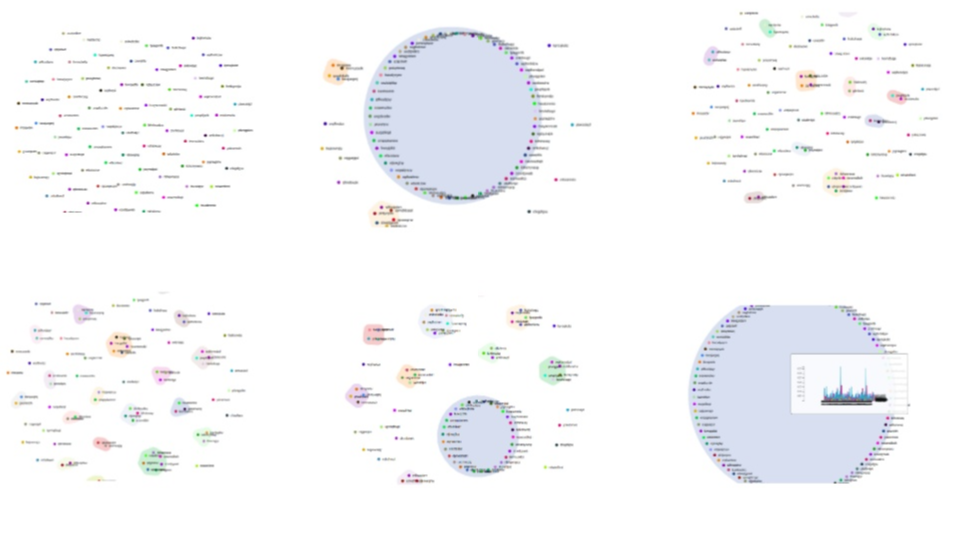
\includegraphics[width=0.80\linewidth]{./image/collage_reticolo-logica(2,4,10).png}
	\caption{Sequenza di creazione del Reticolo della Conoscenza layers(2, 4, 10) - Cluster Based.}
	\label{Sequenza di creazione del Reticolo della Conoscenza layers(2, 4, 10) - Cluster Based.}
\end{figure}
\noindent
\paragraph{Quarta architettura: layers(4, 4, 5, 5)}\mbox{}\\\\
\label{Quarta architettura}
\noindent
Il Reticolo della Conoscenza generato è il seguente:
\begin{figure}[H]
\centering
	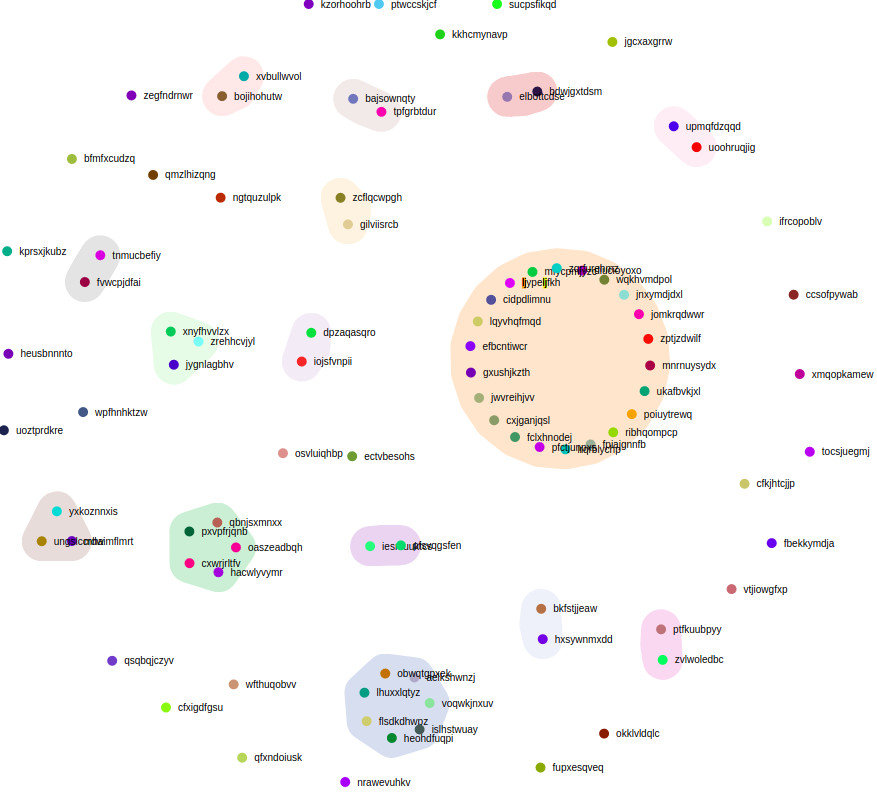
\includegraphics[width=0.70\linewidth]{./image/logica(4,4,5,5).png}
	\caption{Reticolo della Conoscenza layers(4, 4, 5, 5) - Cluster Based.}
	\label{Reticolo della Conoscenza layers(4, 4, 5, 5) - Cluster Based.}
\end{figure}
\noindent

\begin{figure}[H]
\centering
	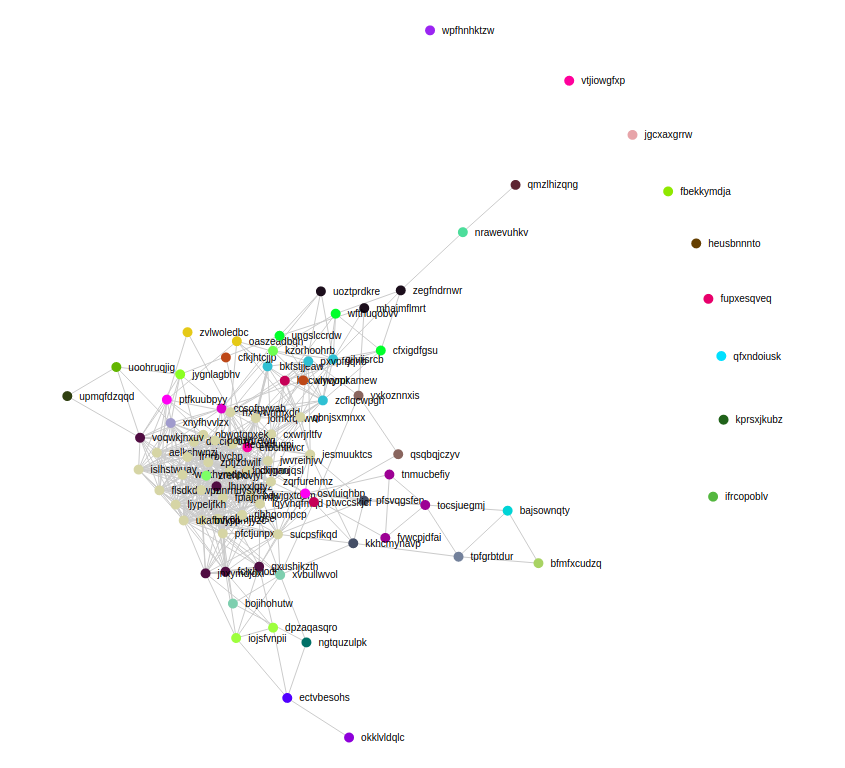
\includegraphics[width=0.70\linewidth]{./image/logica(4,4,5,5)_forced.png}
	\caption{Reticolo della Conoscenza layers(4, 4, 5, 5) - Forced Based.}
	\label{Reticolo della Conoscenza layers(4, 4, 5, 5) - Forced Based.}
\end{figure}
\noindent
\begin{figure}[H]
\centering
	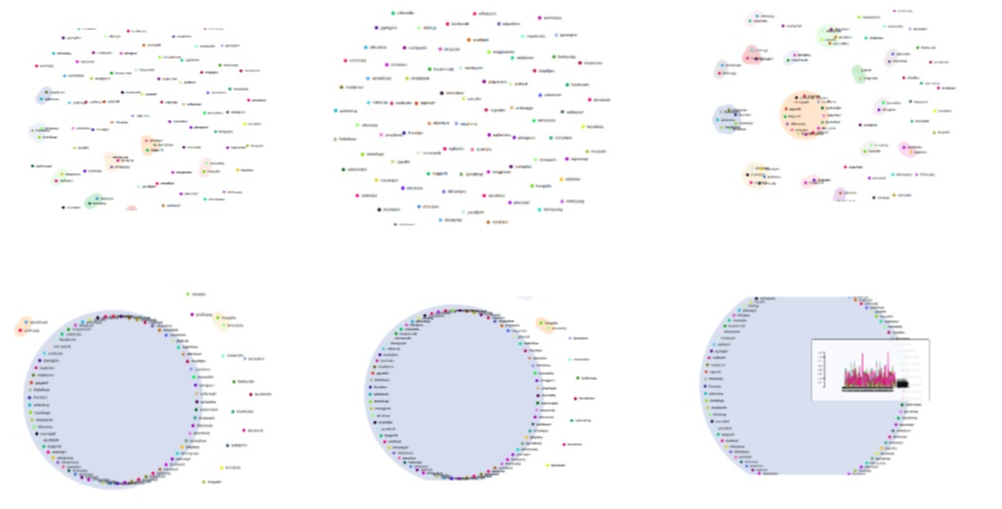
\includegraphics[width=0.70\linewidth]{./image/collage_reticolo-logica(4,4,5,5).png}
	\caption{Sequenza di creazione del Reticolo della Conoscenza layers(4, 4, 5, 5) - Cluster Based.}
	\label{Sequenza di creazione del Reticolo della Conoscenza layers(4, 4, 5, 5) - Cluster Based.}
\end{figure}
\noindent
\subparagraph{Osservazioni dei risultati}\mbox{}
\label{Osservazioni dei risultati}
La seguente architettura ottiene dei risultati discreti.\\
Come si può vedere dalle immagini si ha la presenza di più cluster, uno di dimensione maggiore che progressivamente, con l'incremento della threshold ingloba tutti gli altri gruppi. Tuttavia tale configurazione non vede una distinzione netta di argomento per cluster, però al interno le domande relative alle Serie numeriche e ai diagrammi di Eulero-Venn si mostrano strettamente correlate.
Di seguito descrivo solo alcuni cluser che ritengo significativi.
\begin{longtable}{|c|c|}
	\hline
	\textbf{Serie numeriche} & \textbf{Eulero Venn} \\\hline\hline
	pfctjunpxs & ljypeljfkh \\
	zqrfurehmz & \\
	wqkhvmdpol & poiuytrewq\\ 
\hline
\caption{Domande contenute nel primo cluster}\label{tab:Domande contenute nel primo cluster (rosa)}
\end{longtable}
\noindent
Con riferimento alla figura \ref{Reticolo della Conoscenza layers(2, 4, 10) - Cluster Based.} \textit{poiuytrewq} e \textit{ljypeljfkh} derivano dal medesimo cluster, separati dalle domande sulle serie.
\noindent
Come si può vedere dalle immagini in figura \ref{Sequenza di creazione del Reticolo della Conoscenza layers(4, 4, 5, 5) - Cluster Based.},  alcuni cluster di dimensione ridotta, contengono mini gruppi di domande sulle serie:
\begin{itemize}
\item \textit{zrehhcvjyl} e \textit{xnyfhwlzx};
\textit{pxvpfvjqnb} e \textit{qbnjsxnxx}.
\end{itemize}
\noindent
Sono presenti anche gruppi isolati che mostrano una relazione strettissima tra domande di Serie numerica e di Eulero-Venn.
\begin{itemize}
\item \textit{zcflqcwpgh} e \textit{gilviisrcb};
\item \textit{ccsofpywab} e \textit{xmqopkamew}.
\end{itemize}
\noindent

\subsubsection{Risultati di frequenza sulle domande di logica}
\label{Risultati di frequenza sulle domande di logica}
Per maggiore completezza riporto il Reticolo della Conoscenza generato sulle risposte di frequenza, ai test di logica.
\begin{figure}[H]
\centering
	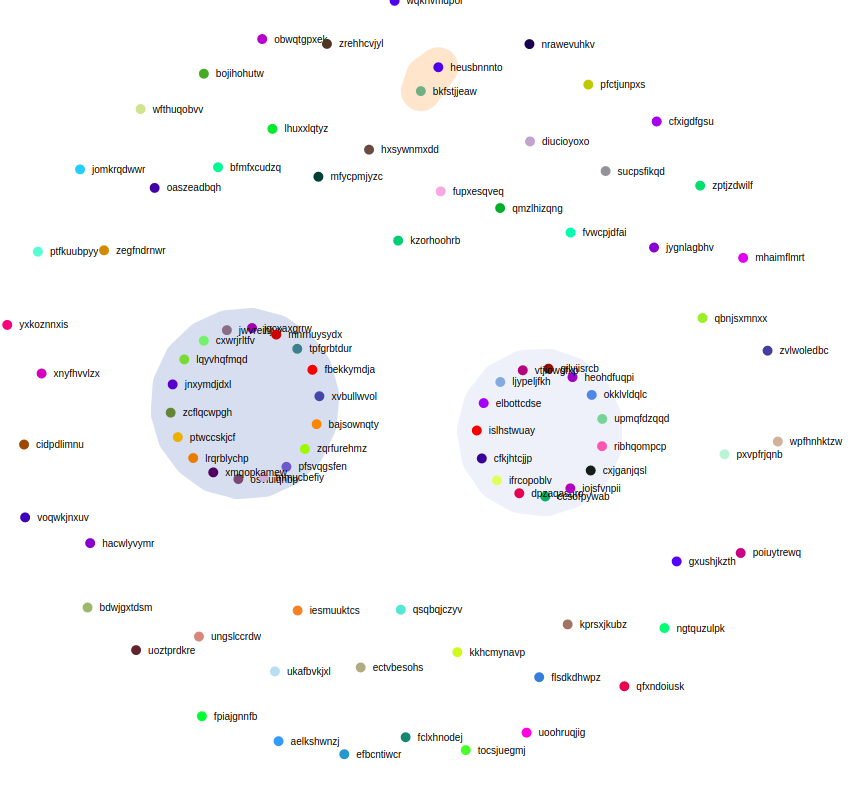
\includegraphics[width=0.70\linewidth]{./image/frequence-logica(4,4,10).png}
	\caption{Reticolo della Conoscenza layers(4, 4, 10) con Frequenza - Cluster Based.}
	\label{Reticolo della Conoscenza layers(4, 4, 10) con Frequenza - Cluster Based.}
\end{figure}
\noindent
La situazione non varia molto rispetto a quanto già incontrato per la Rete di prova. La frequenza tende a smorzare le oscillazioni introdotte dalla probabilità e dalla presenza di risposte non date.\\
Sono individuabili due cluster principali, composti:
\begin{longtable}{|c|c|}
	\hline
	\textbf{cluter 2 (blu scuro} & \textbf{cluster 3 (blu chiaro} \\\hline\hline
	xmqopkamew & gilviisrcb \\
	zqrfurehmz & ccsofpywab \\
	ptwccskjcf & ljypeljfkh \\
\hline
\caption{Domande su Serie numeriche e Eulero-Venn contenute nei cluster}\label{tab:domande su serie e eulero-venn contenute nei cluste)}
\end{longtable}
\noindent
Possono apparire come dei buoni risultati; ma siamo ormai consci dell'impossibilità del metodo statistico di effettuare un calcolo pesato delle risposte alle domande. Tale considerazione non fa altro che invalidare l'uso di questo modello.
\noindent
Inoltre, altra nota dolente, le domande individuate sono molto poche, prima di fondersi in un unico cluster. Invece con l'uso dei dati di previsione, è possibile fare assunzioni sulla difficoltà delle domande (grazie alla presenza di un numero molteplice di cluster contenenti domande delle categorie in esame).


\subsection{Creazione del Reticolo della Conoscenza per delle domande di SQL nel database}
\label{Creazione del Reticolo della Conoscenza per delle domande di sql nel database}
Al termine dello studio e della generazione del Reticolo della Conoscenza per le domande di logica, ho provveduto a generare il Reticolo anche per le domande SQL,  per avere una comprensione maggiore di come il Reticolo si comporta con una variazione del trainset.\\
Le architetture scelte hanno tenuto conto di quanto emerso durante la costruzione dei Reticoli della Conoscenza per le domande di logica.

\subsubsection{Individuazione dei gruppi di argomenti}
\label{Individuazione dei gruppi di argomenti 120}
Le domande SQL, sono domande strutturate nel quale risulta complesso individuare quali siano i macro argomenti; tuttavia nei test presi in esame sono presenti, erroneamente, anche delle domande di Informatica Generale.
\`E dunque lecito ipotizzare che le domande di Informatica Generale compongano dei punti isolati, che saranno gli ultimi a fondersi all'interno del cluster.
\noindent
Di seguito, in forma tabellare viene riportata la categorizzazione delle domande.
\pagebreak
\begin{longtable}{|c|c|}
	\hline
	\textbf{Codice} & \textbf{Argomento} \\\hline\hline
aaxgbiwfen & SQL \\
adiueedxey & SQL \\
afakgklfop & SQL \\
akczmgrdbq & SQL \\
asxurodfne & SQL \\
avagvdjdfu & SQL \\
axrvccwwsp & SQL \\
bbsurwinbt & SQL \\
biweemhojf & SQL \\
blhjkyufeg & SQL \\
bwodxllzmk & SQL \\
bwodxllzmk & SQL \\
csttpqoysn & SQL \\
culepaxyst & SQL \\
cuyddcrymb & SQL \\
cvnhqpgfyp & SQL \\
dagputfvei & SQL \\
dbuqwjsyvj & SQL \\
dkihxiceua & SQL \\
dkzgokqmiq & SQL \\
dlfyuvcbqx & SQL \\
dllpxhzfkt & SQL \\
dzxsvydlth & SQL \\
ebrpcrncwd & SQL \\
eftrkdthng & SQL \\
elqzybkpjl & SQL \\
enitorndkz & Informatica Generale \\
enmkdvzmyk & SQL \\
ewplljreqn & Informatica Generale \\
ffbcwwtnzk & SQL \\
fhqcltuqwl & SQL \\
fjmpjvualm & SQL \\
fkdgytnwzf & SQL \\
fumfugvkrl & Informatica Generale \\
fuzfbwlutx & SQL \\
fyrpicjqan & SQL \\
fzoxjumtyn & SQL \\
gtxwazgyqz & SQL \\
guatssqajf & SQL \\
gyerxpmgqa & SQL \\
hntvpqncrc & Informatica Generale \\
hyfoktjlpp & SQL \\
idfxvfzprt & SQL \\
ieimtqtzpk & SQL \\
iezewxpthv & SQL \\
ifrvxoopny & SQL \\
ifvdeyoyre & SQL \\
ikyqsdhuit & SQL \\
jbpjxhaxyy & SQL \\
jedvsptntk & SQL \\
jycipstmyp & SQL \\
kbnwlxqtqc & SQL \\
kexorxwipq & SQL \\
kfbpwmrkgz & SQL \\
kjecbikedc & SQL \\
kqkjrygfsc & SQL \\
kzzvvwynxn & SQL \\
lgiqayejyf & SQL \\
ljozpygnua & SQL \\
lohspalpqn & SQL \\
lzpqvyslrv & SQL \\
mdwdlplluz & SQL \\
mezjrkwdmi & SQL \\
mligaxxxyv & SQL \\
mljwybuamb & SQL \\
naywhaxocj & SQL \\
nqrcokzyep & SQL \\
oexeosrlxq & Informatica Generale \\
oldnuetsfx & SQL \\
ownmhihmlf & SQL \\
oxinyiwtdw & SQL \\
pdegmbefyz & Informatica Generale \\
pnornaipiy & Informatica Generale \\
pozlktnbwi & Informatica Generale \\
pralrcttdk & Informatica Generale \\
ptfyswhhoi & SQL \\
ptvnijvlyr & SQL \\
qfpxivqgfs & SQL \\
qhpmwyunln & SQL \\
qhurfzksbi & SQL \\
qyfsksfpqr & SQL \\
rcvjbkxijb & Informatica Generale \\
rfveenepae & SQL \\
rjqonwgagd & Informatica Generale \\
rjrbsovupf & SQL \\
rkpyhnweoz & Informatica Generale \\
rlbnjnuraa & SQL \\
rqlhmwvvfr & SQL \\
shwidpusut & SQL \\
slfnwkouex & SQL \\
soaxrpkmyx & SQL \\
tahwadyybr & SQL \\
tmalpukvph & SQL \\
tmptxxfqlg & SQL \\
twjbzfuzhs & SQL \\
uciubnhesv & SQL \\
uctsvufnre & Informatica Generale \\
ukteiawtcu & SQL \\
uoujmoastk & SQL \\
usloxptlnv & SQL \\
vcetherudx & SQL \\
vwesvpdxeu & SQL \\
wbimqkxjpk & SQL \\
wduzcrmbqr & SQL \\
wgqmilmeeo & SQL \\
wqoeigleak & Informatica Generale \\
wyidhotyrc & SQL \\
wyohxxjmbr & SQL \\
xcvjgpwpgd & SQL \\
xdfzuqqaxc & SQL \\
xdpxeikdtg & SQL \\
xxigdvhajv & Informatica Generale \\
xymzioajbw & SQL \\
yjakijsehd & Informatica Generale \\
ynkrhlsqhx & SQL \\
ypvazwngub & SQL \\
yvbkrvodje & SQL \\
zmivrwbcja & SQL \\
zriwusbhcv & SQL \\
zvsnjqiaqb & SQL \\
\hline
	
\caption{Gruppi di argomento per le domande di logica}\label{tab:Gruppi di argomento per le domande SQL}
\end{longtable}
\noindent
\subsubsection{Architettura della Rete testata}
\label{Architettura della Rete testata 120}

\begin{itemize}
\item \begin{verbatim} layer_defs = [];
layer_defs.push({type:'input', out_sx:1, out_sy:1, out_depth:120});
layer_defs.push({type:'fc', num_neurons: 2, activation: 'tanh'});
layer_defs.push({type:'fc', num_neurons: 4, activation: 'tanh'});
layer_defs.push({type:'fc', num_neurons:10, activation: 'tanh'});
layer_defs.push({type:'regression', num_neurons:120});
        
net = new convnetjs.Net();
net.makeLayers(layer_defs);
trainer = new convnetjs.SGDTrainer(net, {learning_rate:0.01, 
momentum:0.1, batch_size:10, l2_decay:0.001});
\end{verbatim}

\item \begin{verbatim}
layer_defs = [];
layer_defs.push({type:'input', out_sx:1, out_sy:1, out_depth:120});
layer_defs.push({type:'fc', num_neurons: 2, activation: 'tanh'});
layer_defs.push({type:'fc', num_neurons: 2, activation: 'tanh'});
layer_defs.push({type:'fc', num_neurons:10, activation: 'tanh'});
layer_defs.push({type:'regression', num_neurons:120});
        
net = new convnetjs.Net();
net.makeLayers(layer_defs);
trainer = new convnetjs.SGDTrainer(net, {learning_rate:0.01, 
momentum:0.1, batch_size:10, l2_decay:0.001});
\end{verbatim}
\end{itemize}
\noindent
\paragraph{Prima architettura: layers(2,4,10)}\mbox{}\\\\
\label{Prima architettura}
\noindent
Il Reticolo della Conoscenza generato è il seguente:
\begin{figure}[H]
\centering
	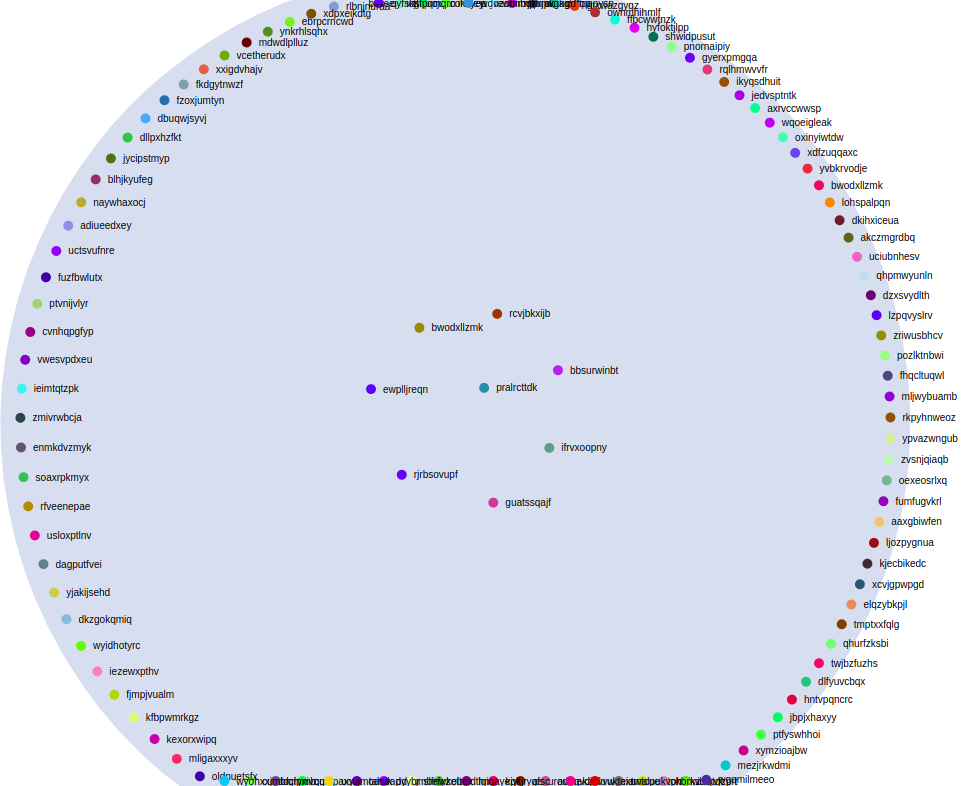
\includegraphics[width=0.70\linewidth]{./image/sql(2,4,10).png}
	\caption{Reticolo della Conoscenza layers(2, 4, 10) - Cluster Based.}
	\label{Reticolo della Conoscenza layers(2, 4, 10) - Cluster Based.}
\end{figure}
\noindent
\begin{figure}[H]
\centering
	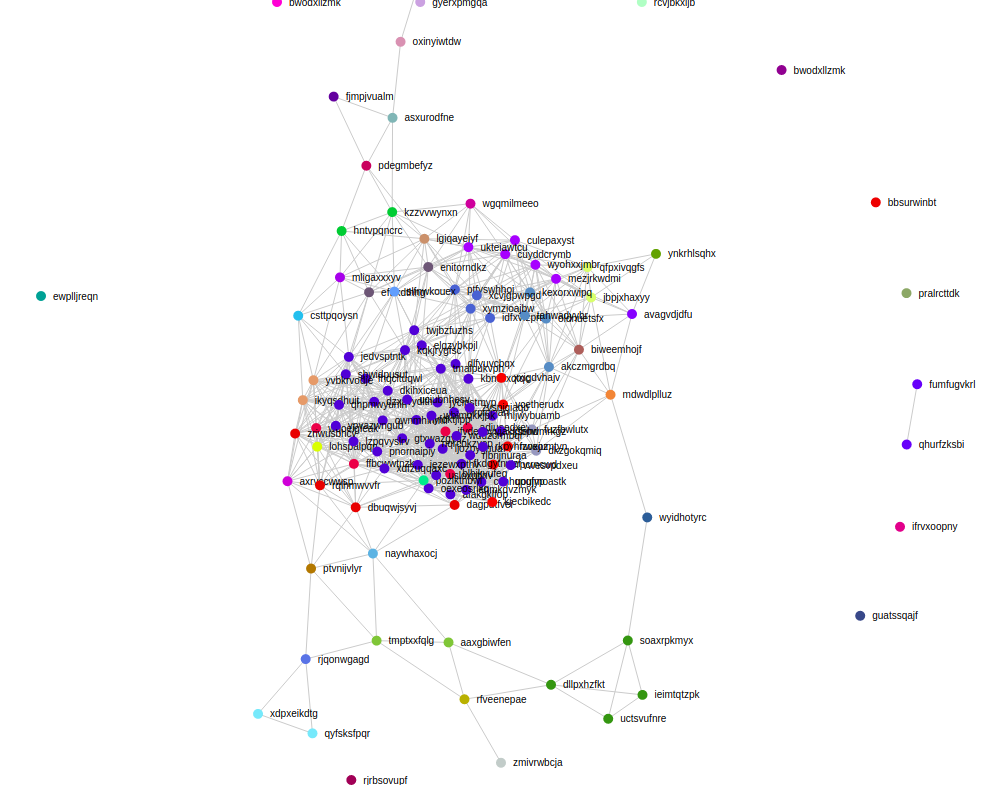
\includegraphics[width=0.70\linewidth]{./image/sql(2,4,10)_forced.png}
	\caption{Reticolo della Conoscenza layers(2, 4, 10) - Forced Based.}
	\label{Reticolo della Conoscenza layers(2, 4, 10) - Forced Based.}
\end{figure}
\noindent

\begin{figure}[H]
\centering
	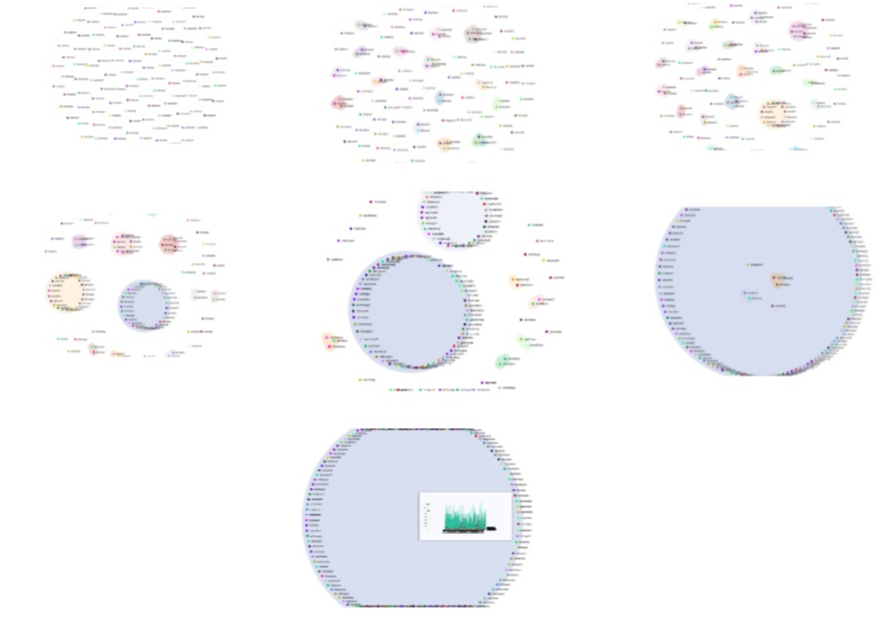
\includegraphics[width=0.70\linewidth]{./image/collage_reticolo-sql(2,4,10).png}
	\caption{Sequenza di creazione del Reticolo della Conoscenza layers(2, 4, 10) - Cluster Based.}
	\label{Sequenza di creazione del Reticolo della Conoscenza layers(2, 4, 10) - Cluster Based.}
\end{figure}
\noindent
\subparagraph{Osservazioni dei risultati}\mbox{}
\noindent
Come si vede dalle immagini appena sopra, le ultime domande ad entrare a far parte del cluster sono:

\begin{longtable}{|c|c|}
	\hline
	\textbf{Codice} & \textbf{Argomento} \\\hline\hline
	ifrvxoopny & SQL \\
	pralrcttdk & Informatica Generale \\
	rcvjbkxijb & Informatica Generale \\
	bwodxllzmk & SQL \\
	ewplljreqn & Informatica Generale \\
	rjrbsovupf & Informatica Generale \\
	guatssqajf & SQL \\
	bbsurwinbt & SQL \\
\hline
	
\caption{Codice delle domande ad essere associate per ultime}\label{tab:codice delle domande ad essere associate per ultime}
\end{longtable}
\noindent
Le domande di Informatica Generale vengono sufficientemente riconosciute dall'architettura come valori anomali.

\paragraph{Seconda architettura: layers(2,2,10)}\mbox{}\\\\
\label{Seconda architettura}
\noindent
Il Reticolo della Conoscenza generato è il seguente:
\begin{figure}[H]
\centering
	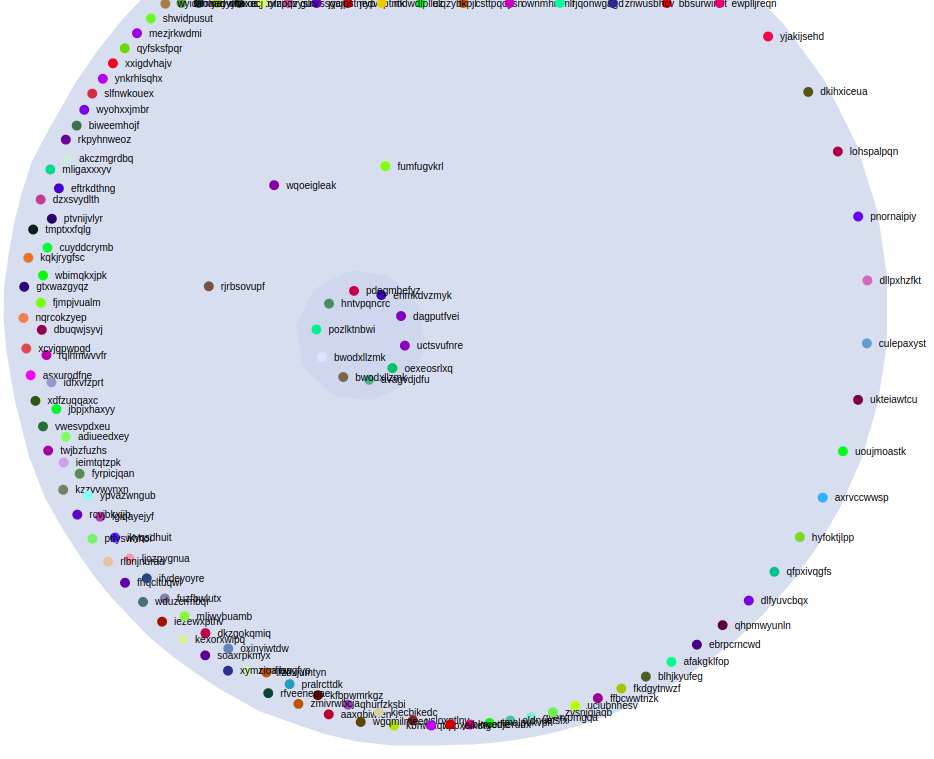
\includegraphics[width=0.70\linewidth]{./image/sql(2,2,10).png}
	\caption{Reticolo della Conoscenza layers(2, 2, 10) - Cluster Based.}
	\label{Reticolo della Conoscenza layers(2, 2, 10) - Cluster Based.}
\end{figure}
\noindent

\begin{figure}[H]
\centering
	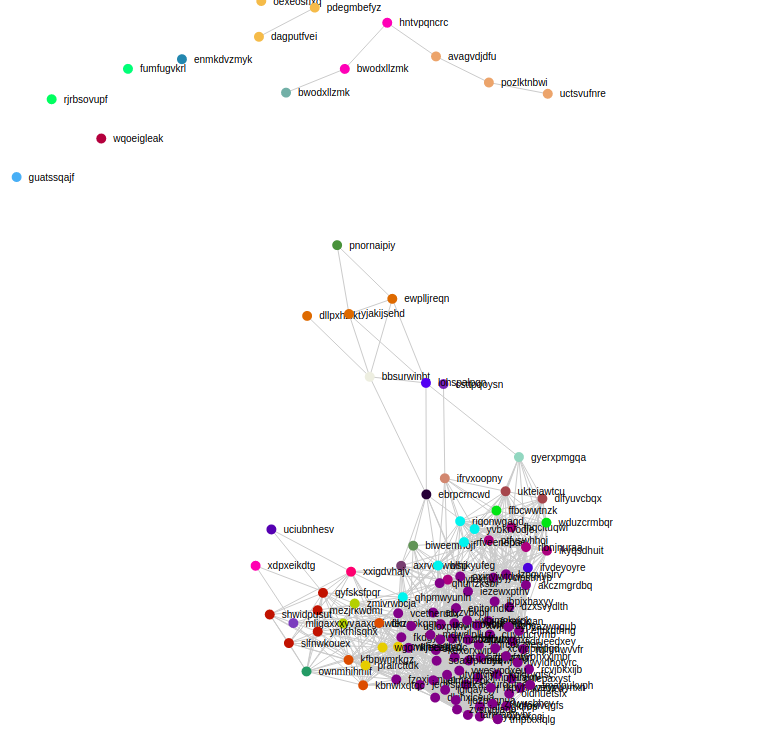
\includegraphics[width=0.70\linewidth]{./image/sql(2,2,10)_forced.png}
	\caption{Reticolo della Conoscenza layers(2, 2, 10) - Forced Based.}
	\label{Reticolo della Conoscenza layers(2, 2, 10) - Forced Based.}
\end{figure}
\noindent

\begin{figure}[H]
\centering
	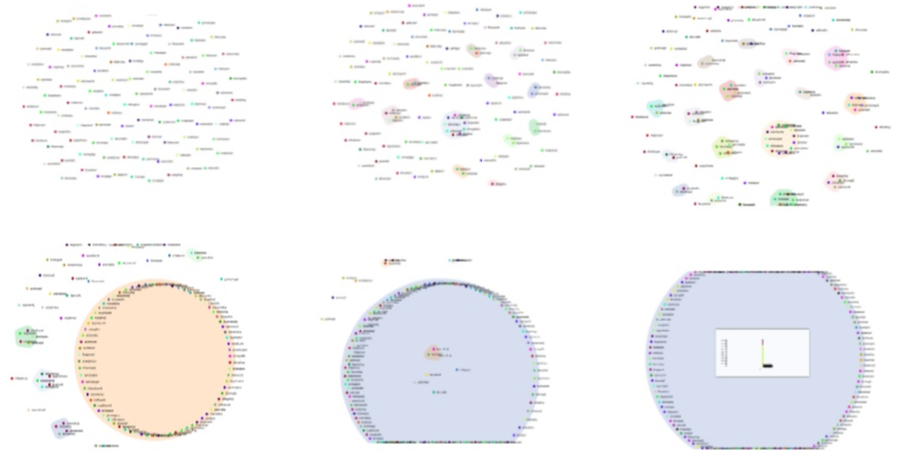
\includegraphics[width=0.70\linewidth]{./image/collage_reticolo-sql(2,2,10).png}
	\caption{Sequenza di creazione del Reticolo della Conoscenza layers(2, 2, 10) - Cluster Based.}
	\label{Sequenza di creazione del Reticolo della Conoscenza layers(2, 2, 10) - Cluster Based.}
\end{figure}
\noindent
\subparagraph{Osservazioni dei risultati}\mbox{}
\noindent
Come si vede dalle immagini appena sopra le ultime domande ad entrare a far parte del cluster sono:

\begin{longtable}{|c|c|}
	\hline
	\textbf{Codice} & \textbf{Argomento} \\\hline\hline
	enmkdvzmy & Informatica Generale \\
	uctssvufnre & Informatica Generale \\
	pdegmbefy & Informatica Generale \\
	pozikthbwl & Informatica Generale \\
	oexeosrxq & Informatica Generale \\
	hntvpqncrc & Informatica Generale \\
	dagputfvei & Informatica Generale \\
	wqoeigleak & SQL \\
	rjbsovupf & SQL \\
	fumfugvkrl & SQL \\
\hline
	
\caption{Codice delle domande ad essere associate per ultime}\label{tab:codice delle domande ad essere associate per ultime}
\end{longtable}
\noindent
Le prime sei domande, contenute in tabella, appartengono ad un singolo cluster, nel quale ne risultano estranee solo le domande \textit{bowdxllzmk} e \textit{avagvdjdfu}, appartenenti alla categoria SQL.
\\
Inoltre vengono associati in relazione stretta:
\begin{longtable}{|c|c|c|}
	\hline
	\textbf{Codice} & \textbf{Argomento} & \textbf{Trattazione del quesito} \\\hline\hline
	\begin{tabular}[c]{cc} oldnuetsfx \\ fyrpicjqan \end{tabular}  & SQL & sargabile \\
	\hline
	\begin{tabular}[c]{cc} usloxptlnv \\ vcetherudx \end{tabular} & SQL & selettività \\
	\hline

\hline
	
\caption{Codice delle domande associate}\label{tab:codice delle domande associate}
\end{longtable}
	
\subsubsection{Risultati di frequenza sulle domande SQL}
\label{Risultati di frequenza sulle domande SQL}
Per maggiore completezza riporto il Reticolo della Conoscenza generato sulle risposte ai test SQL.
\begin{figure}[H]
\centering
	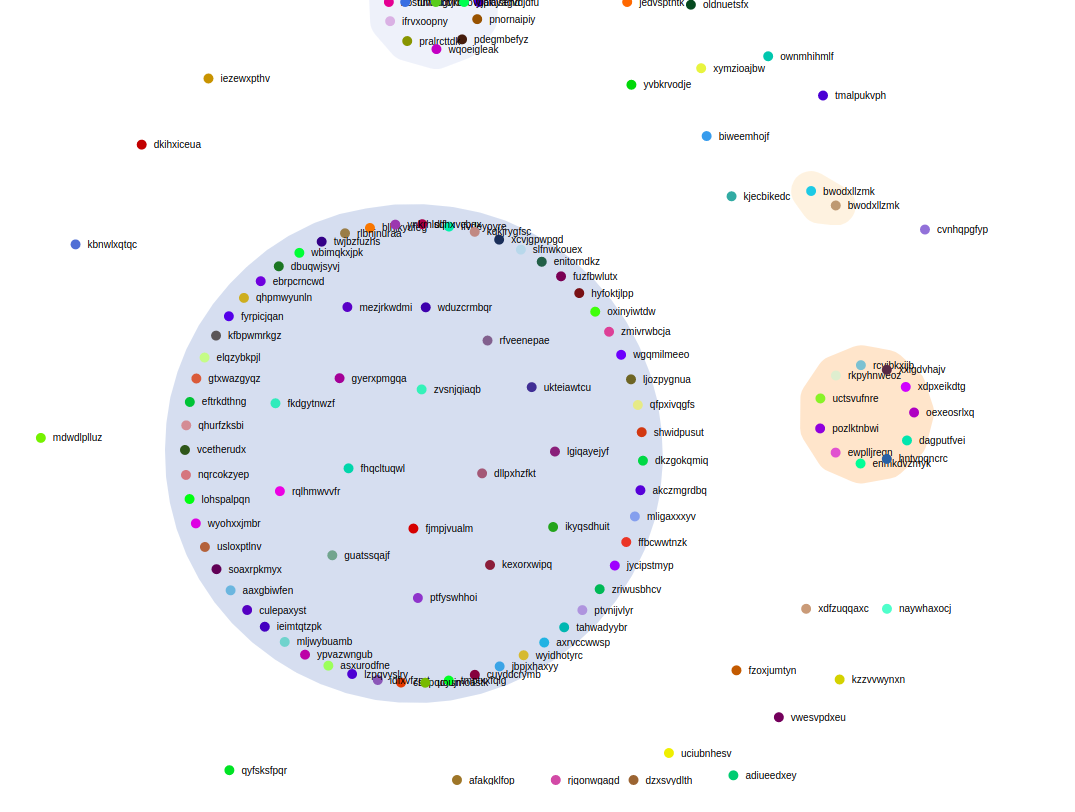
\includegraphics[width=0.70\linewidth]{./image/frequence-sql(2,2,10).png}
	\caption{Reticolo della Conoscenza layers(2, 2, 10) con Frequenza - Cluster Based.}
	\label{Reticolo della Conoscenza layers(2, 2, 10) con Frequenza - Cluster Based.}
\end{figure}
\noindent
Il Reticolo generato dai dati di frequenza rende evidente la non capacità di un solo calcolo statistico di reagire ai valori anomali. Dalla figura sopra, si vede come  le domande di Informatica Generale non vengono individuate e inserite all'interno del Reticolo solo quando si posiziona il threshold al massimo; ma anzi vengono individuate parzialmente, già nei primi stadi di formazione del reticolo, a gruppi in relazione a domande SQL, rientrando fin da subito all'interno del cluster principale.\\
\noindent
Come pro della tecnica di frequenza è l'individuazione immediata di una domanda, \textit{bwodxllzmk}, inserita due volta all'interno del set di dati.

\begin{longtable}{|c|c|}
	\hline
	\textbf{cluter 2 (rosa} & \textbf{cluster 3 (azzurro} \\\hline\hline
	pozlktnbwi & wqoeigleak \\
	ewlplljreqn & pralrcttdk \\
	hntvpqncrc & pnomaipjy \\\
	oexeosrxq & fumfugvkrl \\
	rcvjldkxib & rjrbsovupf \\
    rkpyhnweo & \\
\hline	
\caption{Codice delle domande di logica associate a domande sql}\label{tab:Codice delle domande di logica associate a domande sql}
\end{longtable}
\noindent
Le domande che trattano la sargabilità di un predicato  (\textit{oldnuetsfx}, \textit{fyrpicjgan}, \textit{fuzfbwlutx}), non vengono messo in nessun modo in correlazione dal modello, come invece la Rete neurale effettua.
	
	









